% Setup
\graphicspath{./figures}

\chapter{Experimental Evaluation of Service Mesh systems}
\label{chap:experimental-evaluation}

% Introduction
% - What will this chapter contain and what resaarch question it tries to answer

% Prev chapter -> Design of the benchmark and implementation
% This chapter -> Design of experiments, conducting of experiments and results
In the previous chapter (\cref{chap:system-design}), we defined the \gls{sut} and the metrics that are important to evaluate the performance aspects of \gls{sm} systems. With this in mind, we designed and implemented a tool to benchmark the \gls{sut}. In this chapter, we present the experimental evaluation of \gls{sm} systems using the aforementioned benchmark. With this, we provide an answer to research question \ref{rq-3}. \textit{What are the differences between the different \gls{sm} systems in terms of overhead, throughput and latency?} 


% Rest of the chapter is structured as follows
% - Experimental Setup
% - Experimental Results
% - Analysis/Discussion
The remainder of this chapter is structured as follows. First, in \cref{sec:experiments:design} we introduce the design of the experimental setup. After that, in \cref{sec:experiments:results} we present and explain how to interpret the obtained results. Finally, in \cref{sec:experiments:summary} we discuss the results and their implications.

\section{Experiment Design}
\label{sec:experiments:design}

% The goal of the experimental evaluation


The goal of the experimental evaluation is to gain insights into the performance characteristics of \gls{sm} systems. We do this by designing and conducting experiments to extract and gauge relevant metrics for these systems. This section builds upon the knowledge gained in previous chapters and details all the relevant aspects of the experiments.



\subsection{Service Mesh Selection}
\label{sec:experiments:design:meshes}
% What mesh setups did we choose?
% Why did we choose the service meshes included in the experiments?
% None -> Gives baseline
% Linkerd - Most popular (survey results)
% Istio - Most popular (survey results)
% Traefik - Per node arch
% Cilium - ebpf arch

The selection of \gls{sm} systems to include in the experiments is based on two criteria. First, we aimed to include a representative selection of systems that are used in real-world, production grade environments. Secondly, we aim to include systems based on different architectural approaches. In \cref{chap:survey}, we survey the existing state-of-the-art \gls{sm} systems in the industry and have identified the most frequently used, production grade systems. Furthermore, we identified three different architectural styles that could have major implications on the performance of these systems.

With this in mind we present the list of mesh configurations that is used throughout the experiments.

\begin{enumerate}[label=\textbf{SM\arabic*}, leftmargin=3\parindent]
    \item \textbf{None (baseline)}
    \label{exp:sm:0}
    
    To establish a baseline of performance, we start by performing experiments without any \gls{sm} at all. This enables us to not only compare different mesh systems to one another, but also allows us to paint a picture of the performance overhead compared to an unmeshed environment.
    
    \item \textbf{Istio}
    \label{exp:sm:1}
   
    The first mesh of the selection is \textit{istio}, we chose to include this \gls{sm} because of its prevalence in the industry. During our system survey we have identified that \textit{istio} is the most frequently used, production grade system at the time of writing.
    
    \item \textbf{Linkerd}
    \label{exp:sm:2}
   
    The second mesh of the selection is \textit{linkerd}, we chose to include this \gls{sm} because of its popularity. With a service proxy built for \gls{sm} workloads and a focus on performance, this system quickly gained popularity and established itself as a dominant entry in the industry.

    \item \textbf{Traefik}
    \label{exp:sm:3}
    
    The third mesh included in the experiments is \textit{traefik mesh}. We chose to include this mesh because it uses a vastly different architecture for its data plane. During our system survey we established that most of the identified \gls{sm} systems used a per-service proxy. \textit{traefik mesh} was the only system that we identified that used a \textit{per-node} proxy. By including this mesh in our experiments we aim to uncover the performance implications of this type of configuration.
    
    \item \textbf{Cilium}
    \label{exp:sm:4}
    
    The final mesh included in the experiments is \textit{cilium}. A rather new entry in the world of \gls{sm} systems that we chose to include because of its architecture. During our system survey we identified that \textit{cilium} was the only \gls{sm} system which used a \gls{ebpf} based data plane proxy. By including this mesh in our experiments we aim to expose the performance implications such architecture can introduce.

\end{enumerate}


Additionally, in \cref{tab:experiment:design:mesh} we present the versions used for each \gls{sm} during our experiments.

\begin{table*}[t]
\centering

\begin{tabularx}{\linewidth}{llX}

    \toprule
    Service Mesh       & Version & Reason for inclusion \\
    \toprule
    
    Cilium &
    v1.12.0-rc1 &
    The singular identified \gls{sm} system that uses an in-kernel, \textit{eBPF}-based data plane architecture.
    \\
    
    Istio &
    1.14 &
    Prevalence and market share.
    \\
    
    Linkerd2 &
    2.11.2 &
    Prevalence and market share.
    \\
    
    Traefik Mesh&
    1.4.5 &
    The singular identified \gls{sm} system that uses a per-node service proxy in its  data plane architecture.
    \\
    
    \bottomrule
    
\end{tabularx}

\caption[The \gls{sm} systems used in the experiments.]{The \gls{sm} systems used in the experiments and the reason of inclusion.}
\label{tab:experiment:design:mesh}
\end{table*}




\subsection{Metrics}
\label{sec:experiments:design:metrics}
% - System Resources
% - Throughput
% - Latency

To evaluate the performance characteristics of \gls{sm} systems we have to extract relevant metrics from the \gls{sut}. In \cref{chap:system-design}, we designed and implemented a benchmarking instrument to evaluate \gls{sm} systems. During the requirements analysis (\cref{sec:system:requirements-analysis}) we identified the stakeholders, discussed their use cases and formed a list of requirements. During this, we established a set of metrics that are used to evaluate the performance characteristics based on industry best practices.

Below we present the list of metrics used throughout the experiments

\begin{enumerate}[label=\textbf{M\arabic*}, leftmargin=3\parindent]
    \item \textbf{CPU utilization}
    \label{exp:metric:1}
    
    The first metric that we use during the experiments is related to resource utilization. This helps us to establish how much computational overhead the service proxies of a \gls{sm} introduce. All the CPU utilization results are expressed in fractions of a CPU core per second, e.g. the test system has 2 CPU cores and maximum utilization at a given time would be $2.0$. More specifically, we use the \Verb+container_cpu_usage_seconds_total+ as exposed through the \textit{Kubelet} process and obtain the results through \textit{Prometheus} using the query as seen in Listing \ref{lst:promql-cpu}.
    
    \begin{lstlisting}[caption=PromQL query for CPU metric, label=lst:promql-cpu] 
    sum(rate(
        container_cpu_usage_seconds_total{
            container!="",
            pod=~"(target-fortio|traefik-mesh-proxy|cilium).*"
        }[2s]
    )) by (pod, container)
    \end{lstlisting}

    
    \item \textbf{Memory utilization}
    \label{exp:metric:2}
    
    The second metric that we use in the experiments is also related to the resource utilization. We capture the memory utilization of service proxies by measuring the amount of memory they consume during operation. More specifically, we use the \Verb+container_memory_working_set_bytes+ as exposed through the \textit{Kubelet} process and obtain the results through \textit{Prometheus} using the query as seen in Listing \ref{lst:promql-memory}.
    
    
    \begin{lstlisting}[caption=PromQL query for CPU metric, label=lst:promql-memory] 
    sum(rate(
        container_memory_working_set_bytes{
            container!="",
            pod=~"(target-fortio|traefik-mesh-proxy|cilium).*"
        }[2s]
    )) by (pod, container)
    \end{lstlisting}

    
    \item \textbf{Requests per Second}
    \label{exp:metric:3}
    
    The third metric that we use is the amount of requests the system has handled expressed in requests per second. This metrics allows us to identify to measure the amount of throughput or traffic that a system can handle. 

    \item \textbf{Request Latency}
    \label{exp:metric:4}
    
    The fourth metric that we use in our experiments captures the amount of time it takes for a request to be served. This metric, is expressed as latency in milliseconds allows us to establish the overhead caused in the data path of every request in the system.

\end{enumerate}

In the experiments we do not evaluate metrics related to the resiliency of the system. In our requirements analysis we established a requirement to capture this characteristic based on established best practices. However, is not included in the current experimental design. The reason for this is twofold. First of, we uncovered that the \gls{sm} systems handle timeouts and errors in requests differently \cite{linkerd-retry} and that it involves balancing resiliency capabilities and system load. This means that we cannot compare the systems based on their default settings. Second, to create a fair experiment we have to configure these systems to have identical fault tolerance behaviours, which not all systems support. 


\subsection{Workloads}
\label{sec:experiments:design:workloads}
% GRPC Health
% HTTP echo

The selection of workloads aims to represent varying real-world scenarios that a \gls{sm} might encounter. Since a \gls{sm} handles most, if not all the traffic between software services, it can encounter a wide variety of workloads depending on the use case. With this in mind, we design our experiment to use workloads which are as generic as possible. 

During the systems survey conducted in \cref{chap:survey} we analysed the state-of-the-art \gls{sm} systems and identified their key \glspl{fr} and \glspl{nfr}. We identified that \gls{sm} systems handle service traffic in an application aware manner. Furthermore, we identified the most common application level transport protocols in terms of support. With this in mind, we designed the experiments around the two most common application level protocols. 

\subsubsection{HTTP Workload}
\label{sec:experiments:design:workloads:http}

For the experiments that make use of HTTP workloads we use a simple HTTP service. This service represents a simple echo service and replies with the data a client sends to it. This service requires relatively little system resources to operate and scales well to handle large amounts of connections. Additionally, it is also very configurable which enables us to test HTTP workloads with varying conditions and response payloads.

Although this is a synthetic workload which cannot be compared to any real-world workload, it allows us to capture and evaluate the general performance characteristics of \gls{sm} systems under varying circumstances.

\subsubsection{gRPC Workload}
\label{sec:experiments:design:workloads:grpc}

To evaluate how a \gls{sm} performs under varying application level workloads we included a GRPC workload. During the system survey we observed that all the identified \gls{sm} systems supported the \gls{grpc} protocol and noted that it was a common communication standard in distributed computing. With this in mind we introduced a simple \gls{grpc} based workload. To use the \gls{grpc} protocol, both the client and server need to know the service definition\footnote{\url{https://grpc.io/docs/what-is-grpc/core-concepts/\#service-definition}} since this varies from service to service. Best practices dictate that \gls{grpc} based services should to include a health checking endpoint\footnote{\url{https://github.com/grpc/grpc/blob/master/doc/health-checking.md}}. We use this to our advantage by using a simple \gls{grpc} service that includes this endpoint.

This synthetic workload is used to evaluate the performance implications of other (non-HTTP) application level workloads on \gls{sm} systems.

\subsection{Experimental Environment}
\label{sec:experiments:design:environment}
% Create repeatable experiments
% Cluster/Compute Setup
% Metric Collectors

It is important for experiments to be repeatable and that the variance is a little as possible. This allows others to reproduce and verify the results obtained and therefore be of scientific relevance. 

\subsubsection{Cluster Setup}
\label{sec:experiments:design:environment:cluster}

All the experiments were conducted on a \gls{k8s} cluster running on \gls{gcp}. The cluster was created through their managed \gls{k8s} service \gls{gke}. The decision to use their managed service to construct the cluster was based on their flexible, but vast array of network configuration options. In \cref{tab:experiment:design:cluster-config} we present the most important details of the cluster and node configurations used. Which we will now discuss in further detail.

First, we conducted all the experiments in the \textit{europe-west4} region. More specifically, all the compute nodes are located in the \textit{europe-west4-a} data centre location which is located at Eemshaven in the Netherlands. We chose this location as it was closest to our own location. Secondly, we used the most recent version of \gls{k8s} available at the time of writing in the stable release channel. Thirdly, we made use of \textit{VPC-native-routing}\footnote{\url{https://cloud.google.com/kubernetes-engine/docs/concepts/alias-ips}} which implements the \gls{k8s} networking model\footnote{\url{https://kubernetes.io/docs/concepts/services-networking/\#the-kubernetes-network-model}}. Additionally, we disabled \textit{Dataplane V2} an upcoming networking solution based on \textit{cilium} that would conflict with the \gls{sm} systems that we evaluate.

For the node configurations in the cluster we used a single \textit{e2-standard-2} node. This machine has 2 \textit{vCPUs} and 8 GB of memory\footnote{\url{https://cloud.google.com/compute/docs/cpu-platforms}}. We designed the experiments to be run on a single node cluster to abolish any variance in network latencies during the experiments. If for example, we chose to run the load generator on a single node and the target service on another node we introduce additional variance of network latencies.

\begin{table*}[!t]
\centering

\begin{tabular}{l r}


\toprule
\multicolumn{2}{c}{\textbf{GKE Configuration}}       \\
\toprule

\textbf{Compute Region}    & europe-west4            \\
\textbf{Kubernetes Version}& 1.22.8-gke.201          \\
\textbf{Kubernetes Release Channel} & regular        \\
\textbf{VPC-native-routing}         & enabled        \\
\textbf{Dataplane V2}               & disabled       \\

\toprule
\multicolumn{2}{c}{\textbf{Node Configuration}} \\
\toprule

\textbf{Compute Zone}               & europe-west4-a \\
\textbf{Node Count}                 & 1              \\
\textbf{vCPU}                       & 2              \\
\textbf{Memory}                     & 8 GB           \\  

\bottomrule

\end{tabular}


\caption{The cluster configuration used throughout the experiments.}
\label{tab:experiment:design:cluster-config}
\end{table*}

\subsubsection{Metric Collection}
\label{sec:experiments:design:environment:metric-collection}

We capture two types of metrics from the experiments. The first type of metric is related to the load generator (\ref{exp:metric:3}-\ref{exp:metric:4}). These metrics are collected by capturing the \gls{json} output that the load generator produces. The second type of metric is related to resource utilization (\ref{exp:metric:1}-\ref{exp:metric:2}). To analyse the resource overheads of data plane proxies we have to capture the resource overheads at a fine level of granularity, more specifically, at the level of a \gls{pod}.

To collect resource utilization at this level of granularity we bootstrap the cluster with various monitoring instruments. More specifically, we installed \textit{kube-prom-stack}\footnote{\url{https://github.com/prometheus-community/helm-charts/tree/main/charts/kube-prometheus-stack}}, an end-to-end monitoring solution based on the open-source monitoring solution \textit{Prometheus}\footnote{\url{https://prometheus.io/}}.


\subsection{Experiment Variables}
\label{sec:experiments:design:variables}

When performing load testing experiments we can observe and control many of the variables present in the environment. We can do so on three areas of the benchmark. First of, we can control which \gls{sm} is used, this will be done across all experiment. \cref{sec:experiments:design:meshes} details which \gls{sm} configurations are used and why they were chosen. Additionally, we can control the settings of the load generator. This allows us to tweak what kind of loads we can send (\cref{sec:experiments:design:workloads}) but also control how frequent we send loads and how to handle and or wait for responses. The final area which we can tweak is on the side of the target services. The target services are defined as the receiving endpoints of the load generator. This allows us to adjust the way a service responds, allowing us to introduce artificial delays, introduce faults or change payload sizes.

\begin{table*}[!t]
\centering

\begin{tabularx}{\textwidth}{l X r}

% Header
\toprule
\textbf{Variable}    &
\textbf{Description} &
\textbf{Default}     \\
\toprule

% Values
\textbf{Mesh Configuration} &
What type of \gls{sm} configuration is used in the experiment. (\cref{sec:experiments:design:meshes}) &
- \\

\textbf{Workload Type} &
What type of workload the load generator should send (\cref{sec:experiments:design:workloads}). &
HTTP \\

\textbf{RPS} &
How many requests per second the load generator should generate. &
100 \\

\textbf{Connections} &
Number of simultaneous connections to use when making requests. &
32 \\

\textbf{Duration} &
How long the load generator should generate load to the target service before aggregating and outputting results. &
15 minutes \\

\textbf{Payload Size} &
The size of the response payload in bytes. &
0 \\

\bottomrule

\end{tabularx}

\caption[Overview of the experiment variables.]{Overview of the experiment variables.}
\label{tab:experiment:design:exp-variables}
\end{table*}


In \cref{tab:experiment:design:exp-variables} we present the variables that we control across the experiments in this thesis. Additionally, it includes the default values that were used for these variables if they are not introduced as factor variables within an experiment.

\subsection{Experiments}
\label{sec:experiments:design:overview}

We now introduce the four experiments that were designed and used to evaluate the performance characteristics of \gls{sm} systems. For each of the experiments we introduce their primary goal, discuss how they are executed and reason why we chose this particular design. Additionally, \cref{tab:experiment:design:overview} presents an overview of all the experiments, what type of workloads they use, which  metrics they capture and which factors  are used to control the experiment.

\begin{table*}[!t]
\centering

\begin{tabularx}{\textwidth}{l l l X}

% Header
\toprule
\multicolumn{4}{c}{\textbf{Experiment Overview}} \\
\toprule

% Second Header
\textbf{Experiment}     &
\textbf{Workload}       &
\textbf{Metrics}        &
\textbf{Factors}        \\
\midrule

% Experiments
% \textbf{\ref{exp:design:1}} &
\textbf{EXP 1} &
HTTP                        &
\ref{exp:metric:1}, \ref{exp:metric:2}, \ref{exp:metric:3}, \ref{exp:metric:4}         &
\begin{tabular}{@{}l@{}}
    \textbf{Mesh Configuration} \\
    {}
\end{tabular}
\\
\midrule

% \textbf{\ref{exp:design:2}} &
\textbf{EXP 2} &
HTTP                        &
\ref{exp:metric:1}, \ref{exp:metric:2}, \ref{exp:metric:4}         &
\begin{tabular}{@{}l@{}}
    \textbf{Mesh Configuration} \\
    \textbf{RPS} \textit{(1, 100, 500, 1000)} \\
\end{tabular}
\\
\midrule

% \textbf{\ref{exp:design:3}} &
\textbf{EXP 3} &
HTTP                        &
\ref{exp:metric:1}, \ref{exp:metric:2}, \ref{exp:metric:4}         &
\begin{tabular}{@{}l@{}}
    \textbf{Mesh Configuration} \\
    \textbf{Payload Size} \textit{(0, 1kb, 10kb)} \\
\end{tabular}
\\
\midrule

% \textbf{\ref{exp:design:4}} &
\textbf{EXP 4} &
gRPC                        &
\ref{exp:metric:1}, \ref{exp:metric:2}, \ref{exp:metric:3}, \ref{exp:metric:4}         &
\begin{tabular}{@{}l@{}}
    \textbf{Mesh Configuration} \\
    {}
\end{tabular}
\\
\midrule


      

\end{tabularx}


\caption[Overview of the experiments.]{Overview of the experiments, their metrics and factors.}
\label{tab:experiment:design:overview}
\end{table*}

\begin{enumerate}[label=\textbf{EXP\arabic*}, leftmargin=3\parindent]
    \item \textbf{HTTP Maximum Throughput}
    \label{exp:design:1}
    
    \textbf{Goal} \\
    To find the maximum throughput each of the meshed configurations can achieve.
    
    \textbf{Methodology} \\
    The load generator will run in an unrestricted mode and generate as much load as possible without holding back and without any request timeouts. The maximum throughput is determined by looking at the actual number of requests per second in the configuration was able to achieve.
    
    \textbf{Reasoning} \\
    This experiment will serve as a baseline to determine the maximum throughput of all meshed configurations. The results will be used to determine sensible defaults for the experiments with a pre-defined constant throughput.

    \item \textbf{HTTP Constant Throughput}
    \label{exp:design:2}
    
    \textbf{Goal} \\
    To evaluate how \gls{sm} configurations behave under varying levels of load.
        
    \textbf{Methodology} \\
    The load generator will generate load in a constant and uniform throughput setting. This means that the load generator will produce a set number of requests per second and will not deviate or try to catch up when requests are not processed in time.
    
    \textbf{Reasoning} \\
    This experiment evaluates the \gls{sm} configurations under similar levels of load. This allows us to compare these configurations to one another when they undergo the same workloads.
    
    \item \textbf{HTTP Payload}
    \label{exp:design:3}
    
    \textbf{Goal} \\
    To evaluate how \gls{sm} configurations behave with varying payload sizes.

    \textbf{Methodology} \\
    The load generator will produce HTTP requests to the target service, which in turn will respond with pre-determined payload sizes.

    \textbf{Reasoning} \\
    This experiment introduces several pre-determined payload sizes to evaluate the effects of additional application data being transferred in meshed environments. This allows us to study the effects and potential additional overheads extra data transfers may cause. 
        
    \item \textbf{gRPC Maximum Throughput}
    \label{exp:design:4}
    
    \textbf{Goal} \\
    To evaluate how meshed configurations behave with alternative communication protocols.
        
    \textbf{Methodology} \\
    The load generator will generate gRPC traffic towards the gRPC service and do so in an unrestricted manner, meaning it will try to generate as much load as possible without holding back and without enforcing any timeouts. The maximum throughput is determined by looking at the actual number of requests per second in the configuration was able to achieve.
    
    \textbf{Reasoning} \\
    This experiment allows us to evaluate the effects of alternative application level protocols. During the system survey we uncovered that \gls{sm} systems inspect and use this data to for both observability and routing functionalities. This experiment allows us to uncover the effects of alternative, but common, application level protocols widely used within the industry.

\end{enumerate}


\section{Experiment Results}
\label{sec:experiments:results}

In this section, we present the results obtained from the experiments as defined in \cref{sec:experiments:design:overview}. We first present the main findings in \cref{sec:experiments:main-findings}. After this, we present and explain how to interpret the results per experiment in \cref{sec:experiments:results:per-experiment} and discuss these findings in greater detail.

\subsection{Main Findings}
\label{sec:experiments:main-findings}
% Significant decrease in throughput
% Additional avg latency, esp tail ends. p99+
% Traefik experiences bottlenecks, bimodal distribution
% Istio consumes most CPU resources
% Applications Payloads seem to have little effect on performance
% Application protocol seems to have little impact, although linkerd performs a bit worse on gRPC throughput
% Traefik failed to handle gRPC worklaods
% Cilium best allround performer

We now present the main findings of the conducted experiments.

\begin{enumerate}[label=\textbf{MF\arabic*}, leftmargin=3\parindent]
    \item \textbf{There can be a significant drop in maximum throughput when using a service mesh}
    \label{exp:mf1}
    Every service mesh suffers from a decrease in maximum throughput. The observed decrease in throughput varies greatly, with a best-case scenario having a  $-16.8\%$ decrease while the worst performing configuration has a significant  $-97.38\%$ decrease in maximum throughput.
    
    \item \textbf{There can be a significant increase in request latencies when using a service mesh}
    \label{exp:mf2}
    A service mesh introduces additional request latency by introducing a network proxy in front of the service. This additional overhead, however, can have a large impact on average and tail end request latencies as observed. With the best performing mesh increasing the average request latency with $20.27\%$ whereas the worst performing configuration saw a staggering $3720.95\%$ uplift.
    
    \item \textbf{Traefik mesh experiences bottlenecks after it reaches a certain throughput threshold}
    \label{exp:mf3}
    We observed that \textit{Traefik} cannot perform above a certain throughput level, and will throttle requests, resulting in a bimodal distribution of request latencies and a significant loss of performance for those requests.
    
    \item \textbf{Istio is the most demanding in terms of CPU utilization}
    \label{exp:mf4}
    We observe that \textit{Istio} consumes significantly more CPU resources compared to other configurations. We also observe that this is due to its data plane proxy which does not scale as well as the proxies in other configurations.
    
    \item \textbf{Application payloads have little to no effect on the observed performance}
    \label{exp:mf5}
    We observed that increasing the application payload, has little to no effect on the performance of meshed configurations.
    
    \item \textbf{Application level protocols have little to no effect on the observed performance}
    \label{exp:mf6}
    We observed that different layer 7 protocols, HTTP vs gRPC, had little to no impact on the decrease in throughput observed.
    
    \item \textbf{Traefik was unable to handle gRPC workloads}
    \label{exp:mf7}
    We observed that \textit{Traefik} was unable to handle and execute gRPC workloads in our experiments even though it listed explicit support for gRPC.
    
    \item \textbf{Cilium was the best all-round performing configuration, with a significant margin}
    \label{exp:mf8}
    We observed that the configuration using \textit{Cilium} outperformed any other configuration using a \gls{sm} with significant margins in all the experiments that were conducted.
\end{enumerate}



\subsection{Results per Experiment}
\label{sec:experiments:results:per-experiment}

We now present the results of each individual experiment and discuss how to interpret them.

\subsubsection{\ref{exp:design:1} - HTTP Maximum Throughput}
\label{sec:experiments:results:per-experiment:01}
% Goal:
% To find the maximum throughput each of the meshed configurations can achieve.

% Introduce all figures
The goal of the first experiment was to determine the maximum throughput of each meshed configuration. The results of this experiment are depicted in \cref{fig:exp:result:01:latency}, \cref{fig:exp:result:01:cpu} and \cref{fig:exp:result:01:memory}. 

% Histogram results
% How to read results
The first illustration (\cref{fig:exp:result:01:latency}), depicts a histogram that shows the distribution of request latencies for each meshed configuration. The x-axis represents the latency expressed in milliseconds in a logarithmic fashion. The left y-axis is related to the bars in the histogram and represents the number of requests. The right y-axis is related to the cumulative density function line (the yellow line on top of the histogram) and represents the proportion of requests. Each bar represents a bin of the histogram, and all bins in the histogram can be of varying sizes. The bins closer to the expected latency are smaller, whereas bins further away from the expected latency can cover larger areas. Additionally, each plot in the figure is accompanied by descriptive statistics such as the minimum, average and maximum request duration. Furthermore, it also contains the achieved throughput, expressed as requests per second (\textbf{RPS}).


\begin{figure}[!t]
    \centering
    
    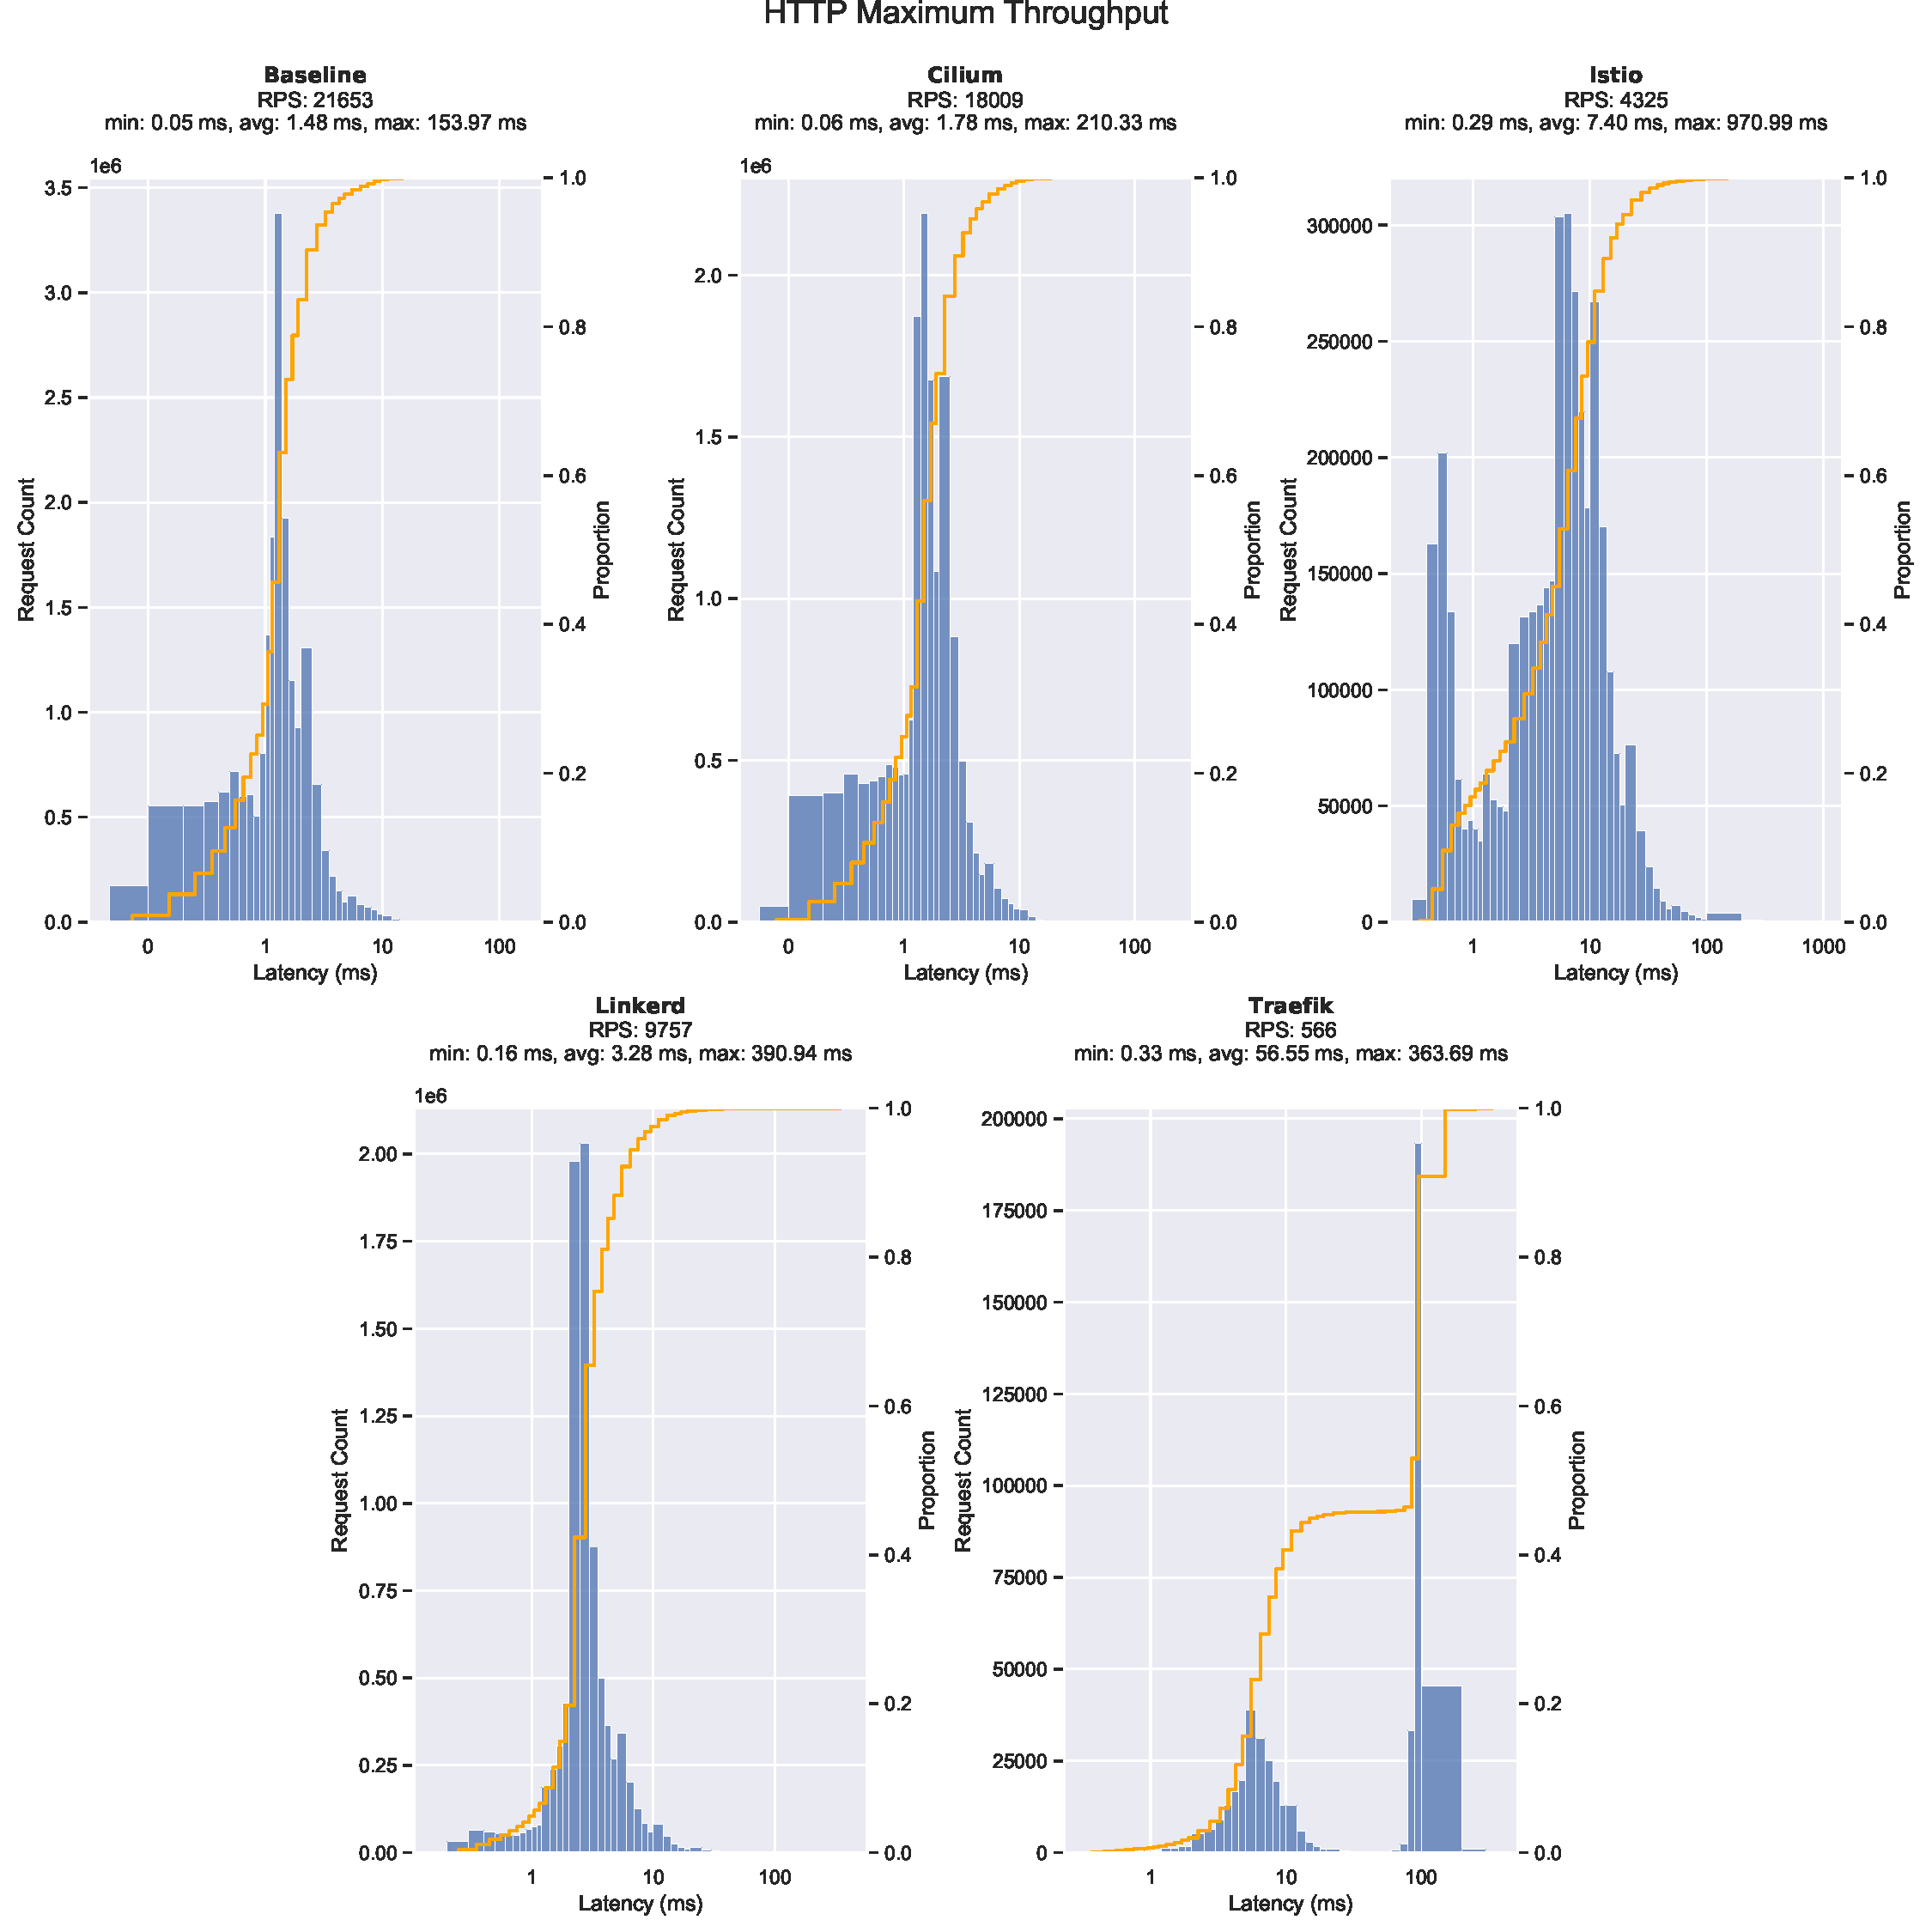
\includegraphics[width=\linewidth]{5_experimental_evaluation/figures/exp_01-latency-results.pdf}

    \caption{\ref{exp:design:1} - Latency Results}
    
    \label{fig:exp:result:01:latency}
\end{figure}



% Findings
% - Baseline best (highest RPS, best latency avg)
% - Distributions roughly normal
% - Large increases in average/tail end latencies
% - Traefik mesh bimodal distribution
% cilium QPS diff: -16.827679769486704%
% istio QPS diff: -80.0264142981776%
% linkerd QPS diff: -54.940993873502805%
% traefik QPS diff: -97.38692130213765%
From the histograms in \cref{fig:exp:result:01:latency} we can observe that the baseline performs the best, i.e. it has the highest observed throughput and the minimum, average and maximum latencies outperform any meshed configuration. In terms of achieved throughput, \textit{Cilium} performs second best and loses $-16.83\%$ compared to the baseline configuration with no \gls{sm} applied. The configuration using \textit{Linkerd}, however, lost more than half ($-54.94\%$), whereas the situation for \textit{Istio} and \textit{Traefik} was even worse as they saw a throughput drop of $-80.26\%$ and $-97.39\%$ respectively. Another interesting observation can be made when looking at the average latencies and tail end latencies for the meshed configurations compared to the baseline measurements. First, we can see a minor increase in average latency for \textit{Cilium}. More interestingly, however, we can see a $+121.62\%$ increase for the \textit{Linkerd} configuration compared to the baseline. The results for the \textit{Istio} configuration is even worse, where it sees an uplift of $+400\%$ for the average request latency compared to the baseline. \textit{Traefik}, however, sees the largest increase with a massive $+3720.95\%$ uplift in average request latency. When taking a closer look at the distributions in the histograms we can also notice that the configuration using the \textit{Traefik} mesh has a bimodal distribution, where one mode is around 8 milliseconds and another mode exists around the 100 millisecond mark.

% Explanation CPU/Mem line plots
In \cref{fig:exp:result:01:cpu} and \cref{fig:exp:result:01:memory} we depict the CPU and memory utilization results of the experiment. Both illustrations come in the form of line plots that have their metric expressed on the y-axis, for the CPU usage this is represented as fractions of a CPU core for both user and kernel time and for the memory utilization this is expressed in kilobytes used. On the x-axis we depict the time delta of the experiment since the start in minutes, each experiment takes 15 minutes and the lines in the plot show the resource utilization values over time. Additionally, each plot can have multiple lines, with one line for each container relevant to the configuration. In other words, we track the resource utilization for the containers related to the data path of the network traffic. In the baseline configuration this is only one experiment, since it does not employ a \gls{sm}, but in the meshed configurations proxy containers are plotted as well as indicated by the legends above the figures.

\begin{figure}[!t]
    \centering
    
    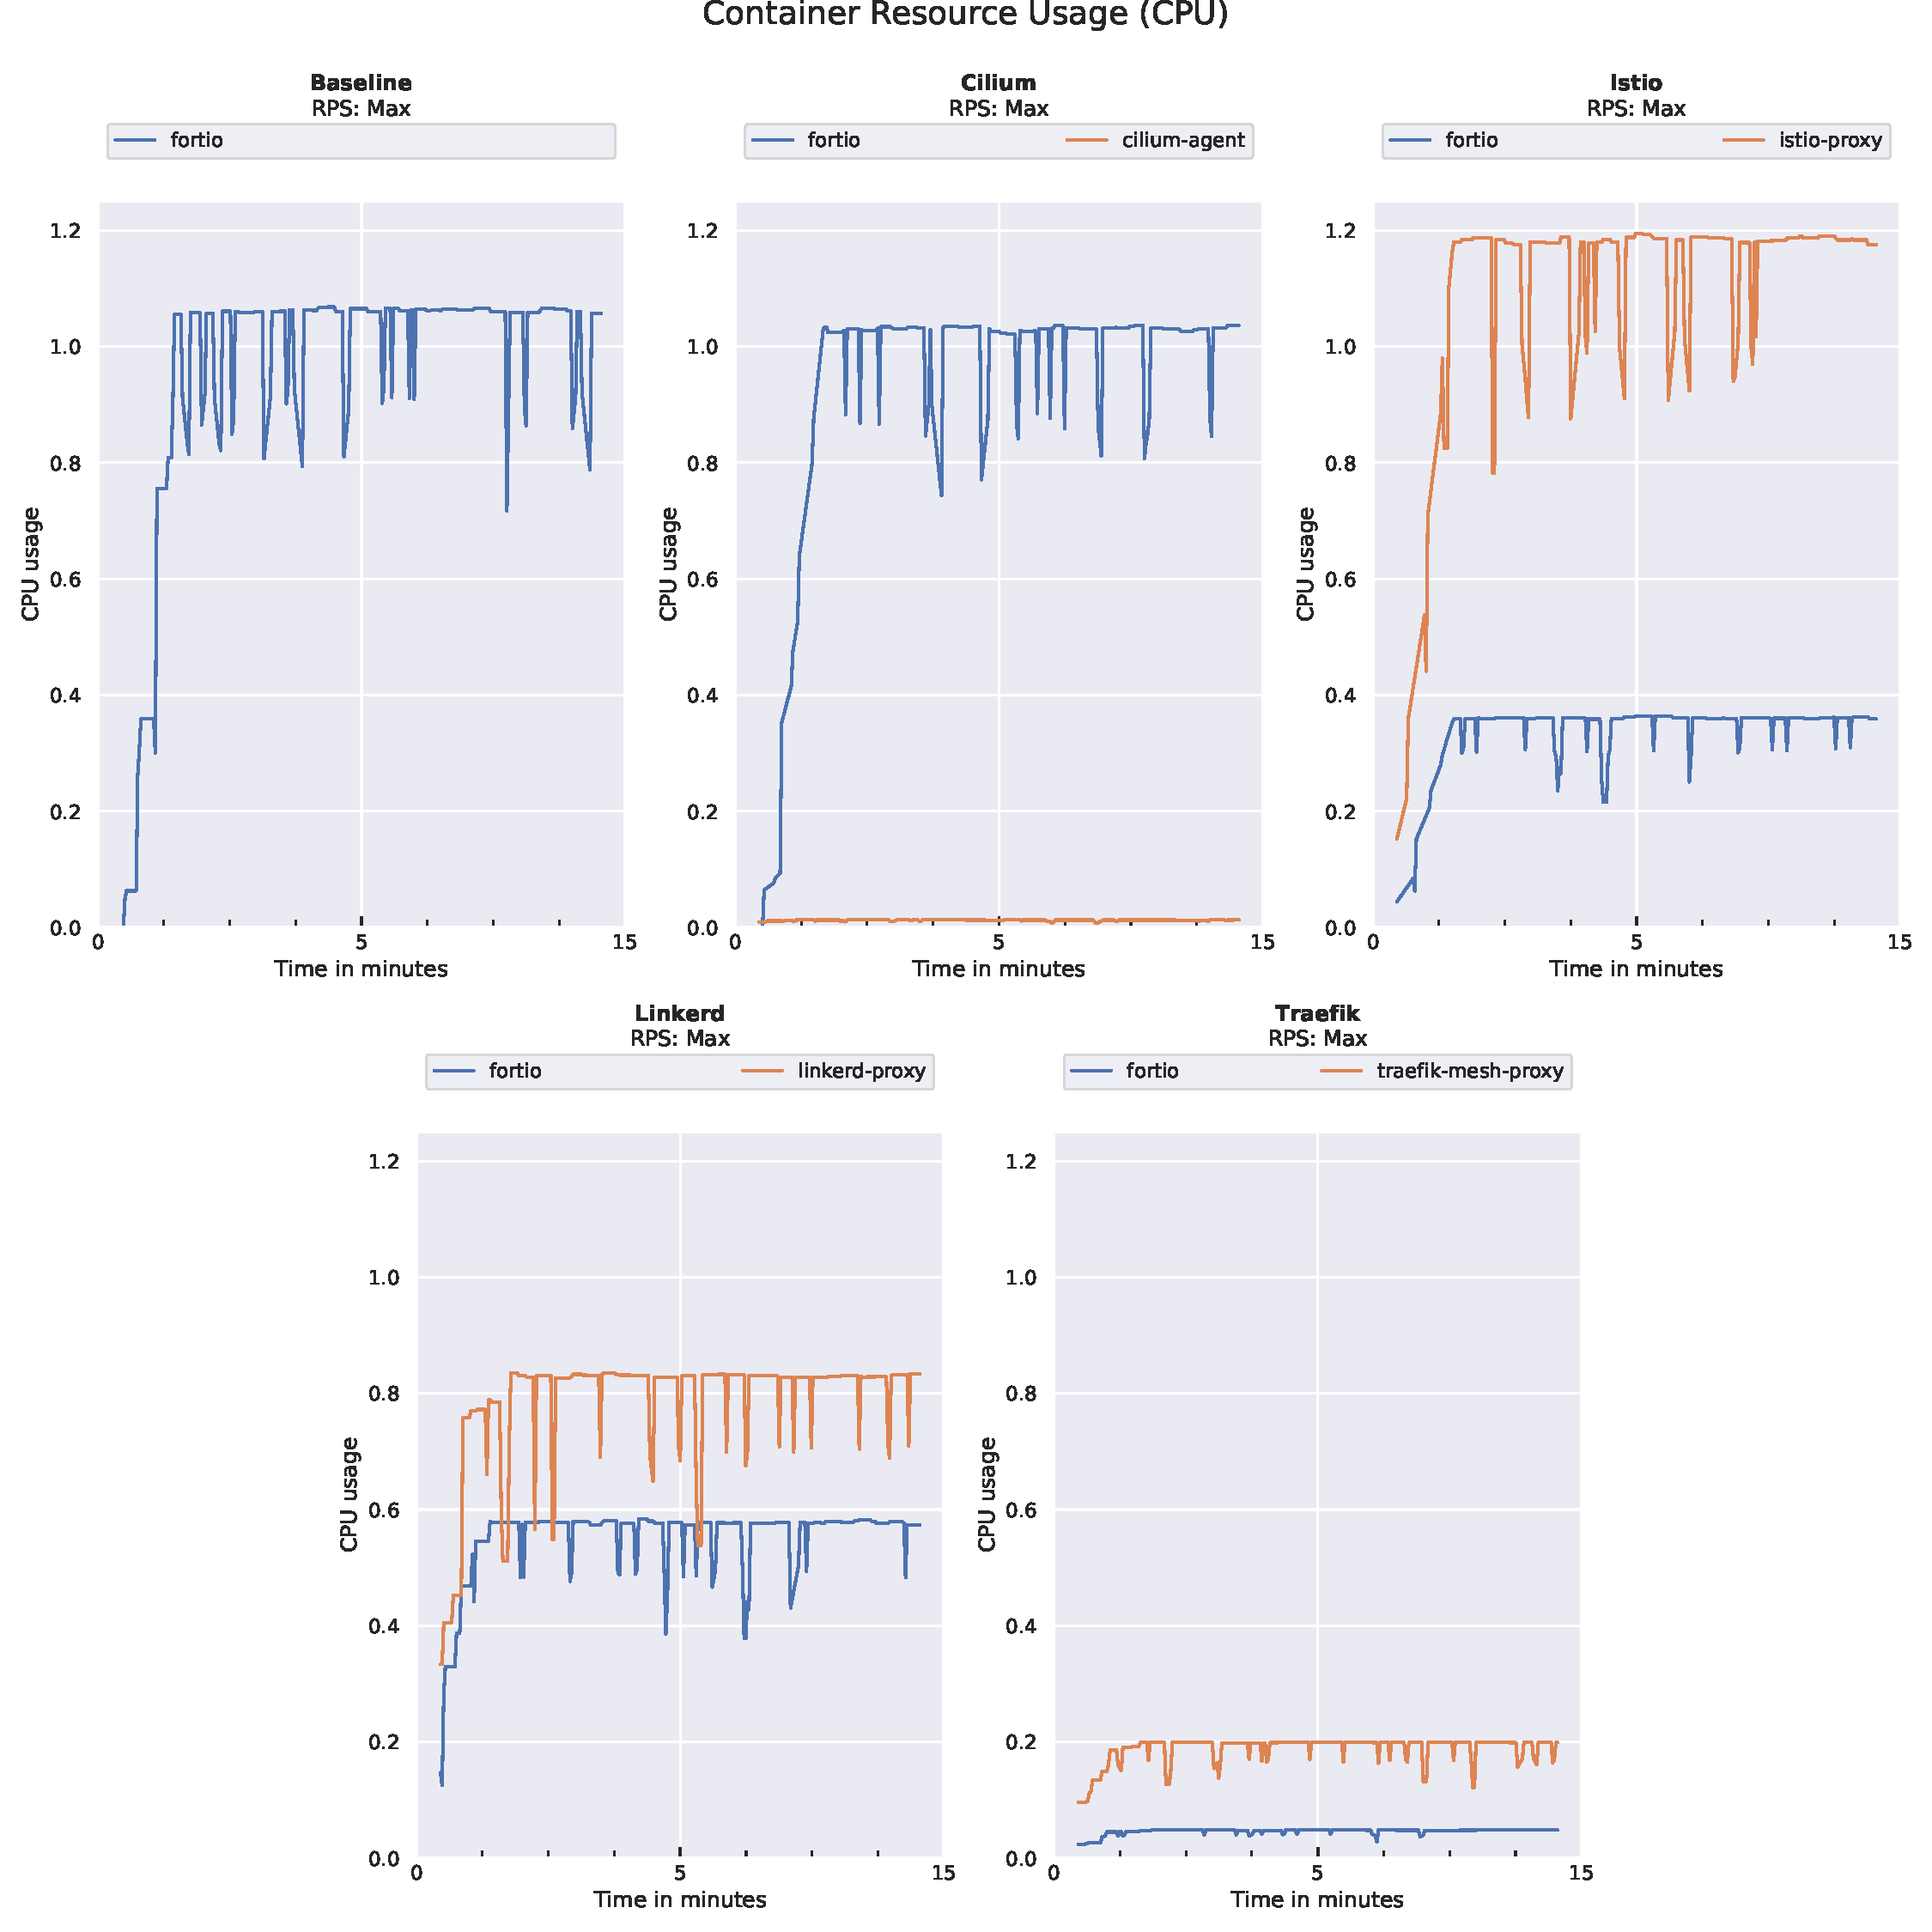
\includegraphics[width=\linewidth]{5_experimental_evaluation/figures/exp_01-cpu-results.pdf}

    \caption{\ref{exp:design:1} - CPU utilization results.}
    
    \label{fig:exp:result:01:cpu}
\end{figure}


% Notable findings
% Small rampup time
% 'fortio' usage -> RPS
% Istio-proxy high utilization
% Linkerd less, but more throughput
% Cilium very low utilization
% Traefik low -> bottleneck?
From the line plots in \cref{fig:exp:result:01:cpu} we can observe that for each configuration there is a small ramp-up time until the CPU utilization settles in. Furthermore, we can observe and relate back to our results depicted in the histograms (\cref{fig:exp:result:01:latency}) that there is a direct correlation between CPU utilization and throughput for the \textit{fortio} container (the target service that represents an echo server), as the meshed configurations that achieved less throughput have an inverse relation on CPU utilization. Interesting observations can be made regarding the CPU utilization of the service proxies. First of, \textit{Cilium}, with their kernel based proxying solution (\cref{{sec:survey:results:comparison:proxy}}) seems to have very little overhead compared to other proxying solutions. Second, the proxy used in the \textit{Istio} configuration appears to have the highest overhead, taking up more than an entire CPU core. Additionally, the proxy used in the \textit{Linkerd} configuration uses less CPU resources, which indicates that this solution is more efficient than \textit{Linkerd}'s proxy as it was able to handle a higher throughput as well. Finally, we observe that the \textit{Traefik} configuration used very CPU little resources at all, indicating bottlenecks of some sort.

From the plots depicting memory consumption in \cref{fig:exp:result:01:memory} we can see that for each configuration the memory usage was very minimal. The \textit{cilium-agent} container reached a spike and consumed at most $2.27$MB during maximum load. This amount is negligible for most systems and indicates that the data path proxies will likely not be memory constrained.

\begin{figure}[!t]
    \centering
    
    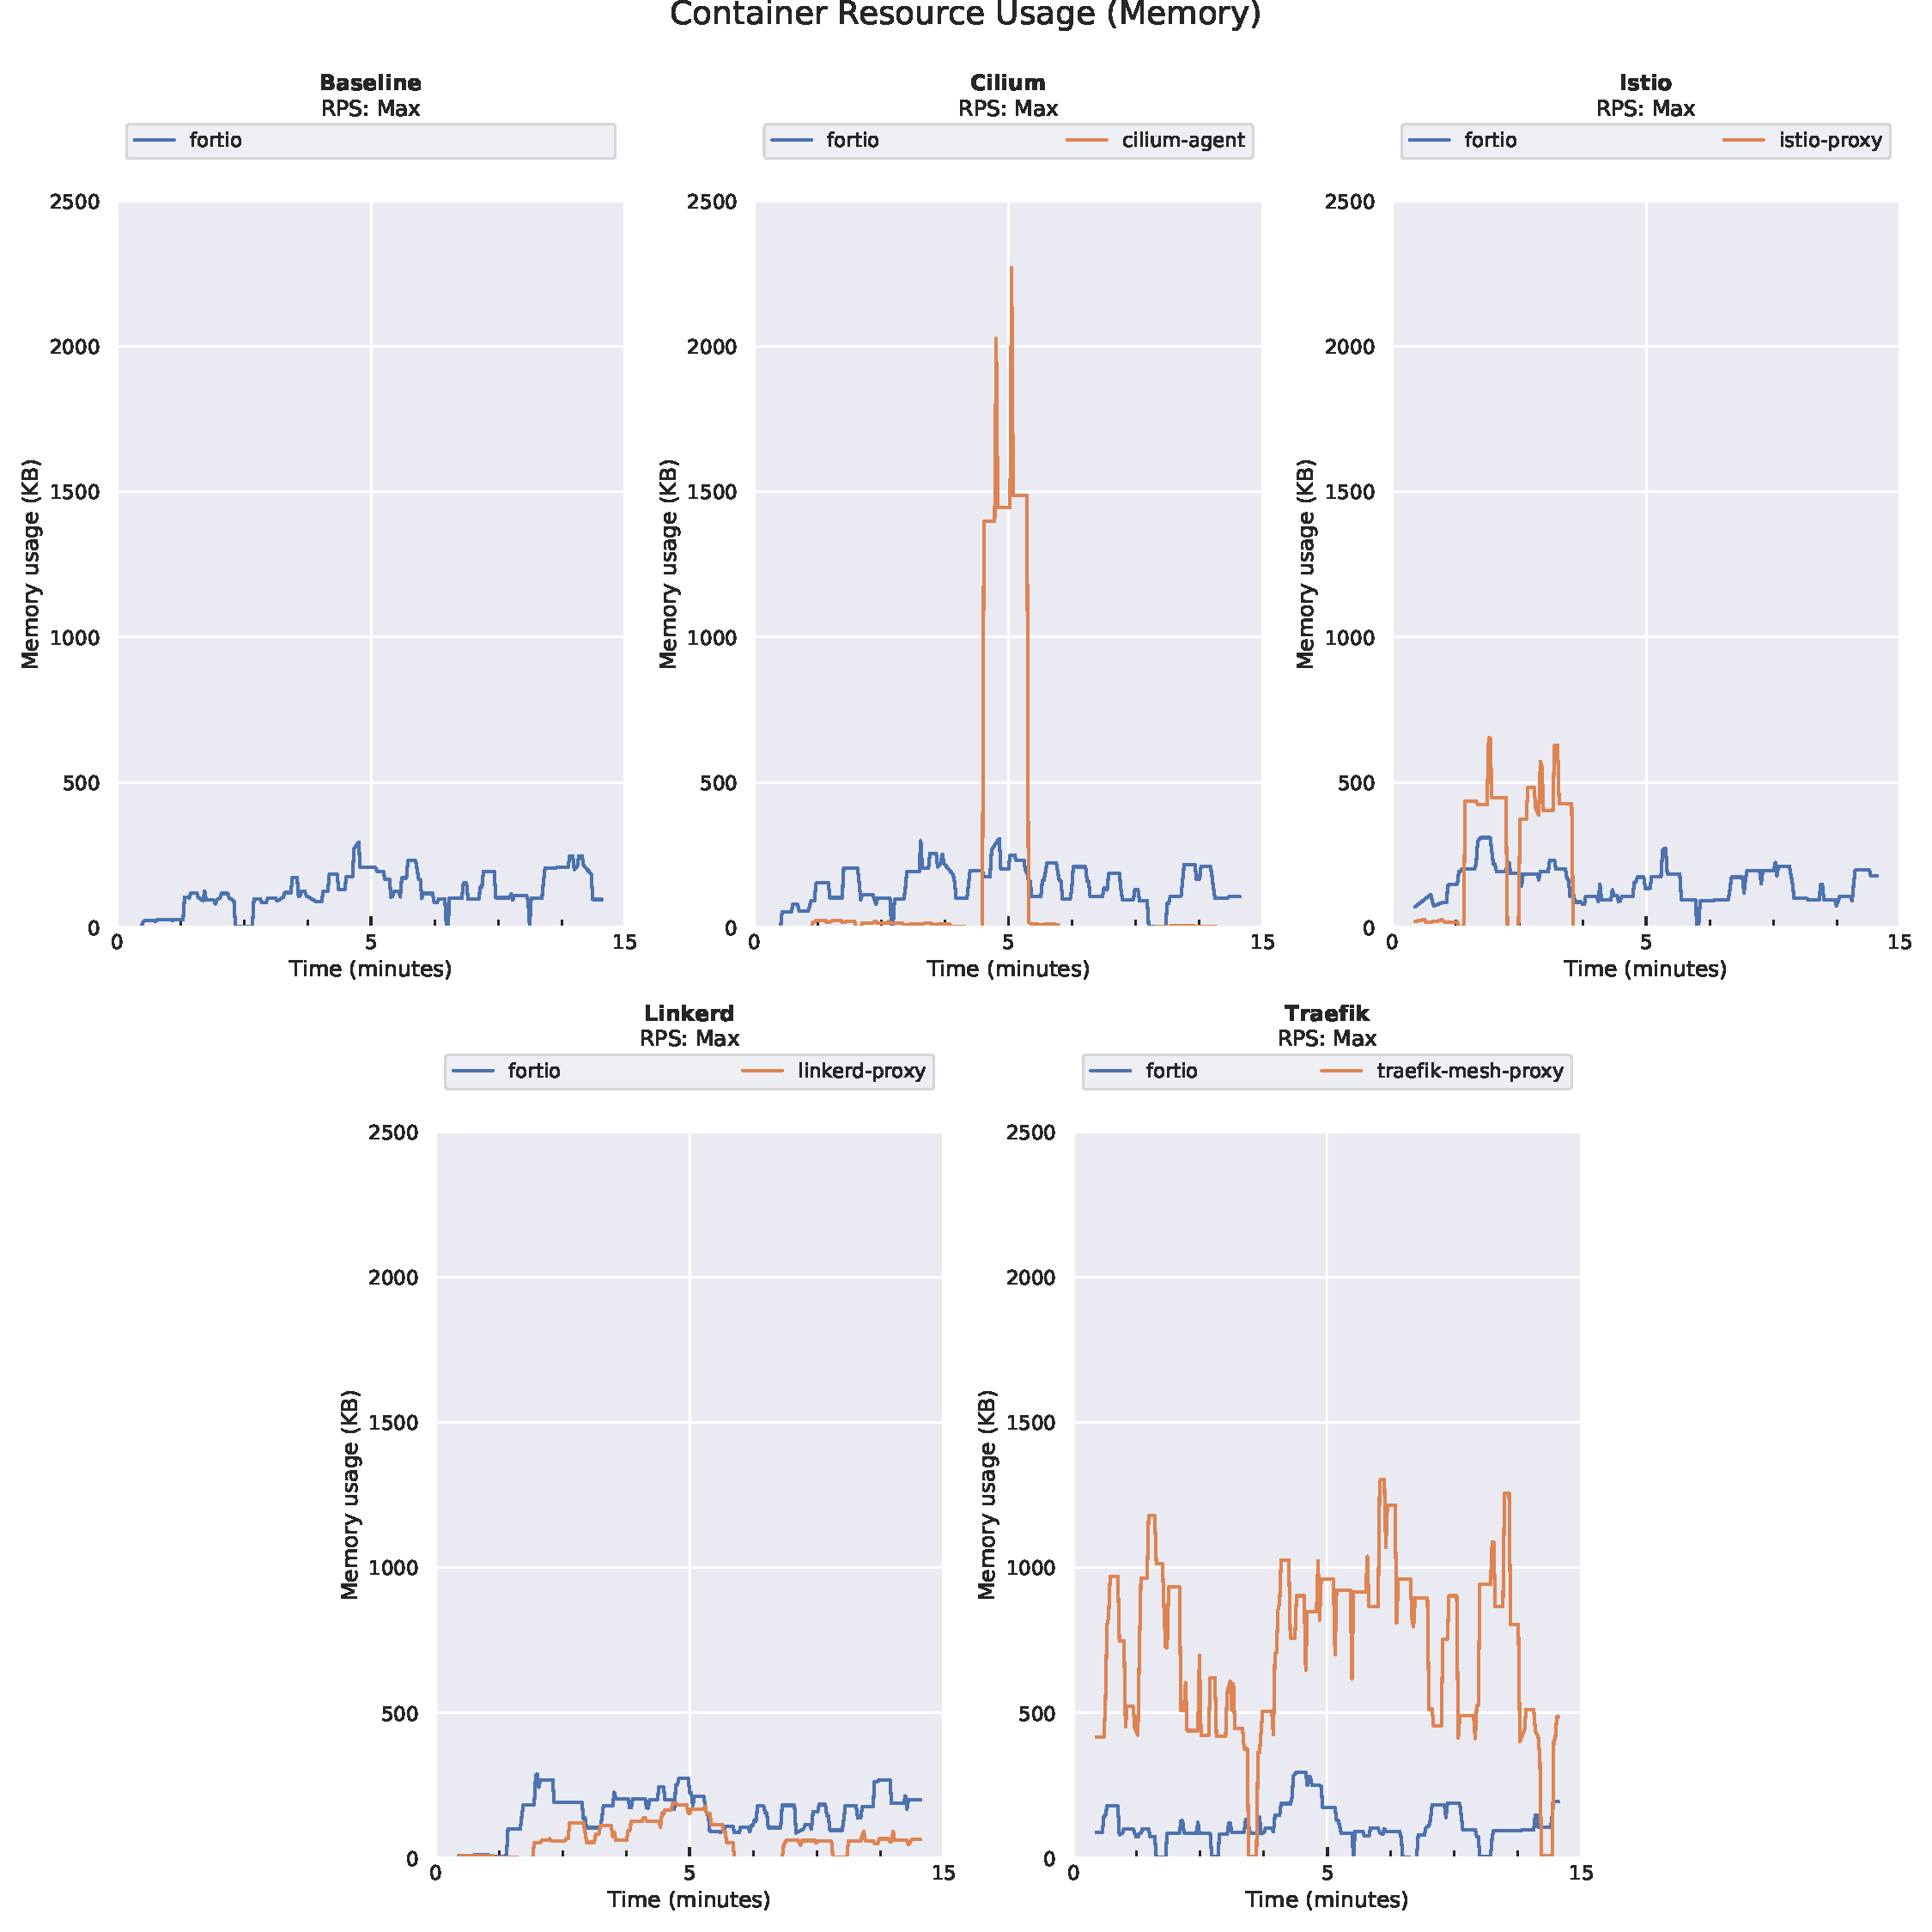
\includegraphics[width=\linewidth]{5_experimental_evaluation/figures/exp_01-memory-results.pdf}

    \caption{\ref{exp:design:1} - Memory Results}
    
    \label{fig:exp:result:01:memory}
\end{figure}



\subsubsection{\ref{exp:design:2} - HTTP Constant Throughput}
\label{sec:experiments:results:per-experiment:02}
% Goal: To evaluate how \gls{sm} configurations behave under varying levels of load.

The second experiment had as goal to evaluate the different \gls{sm} configurations under predefined levels of constant throughput. The results of this experiment are depicted in \cref{fig:exp:result:02:latency}, \cref{fig:exp:result:02:cpu} and \cref{fig:exp:result:02:memory}.


\begin{figure}[!t]
    \centering
    
    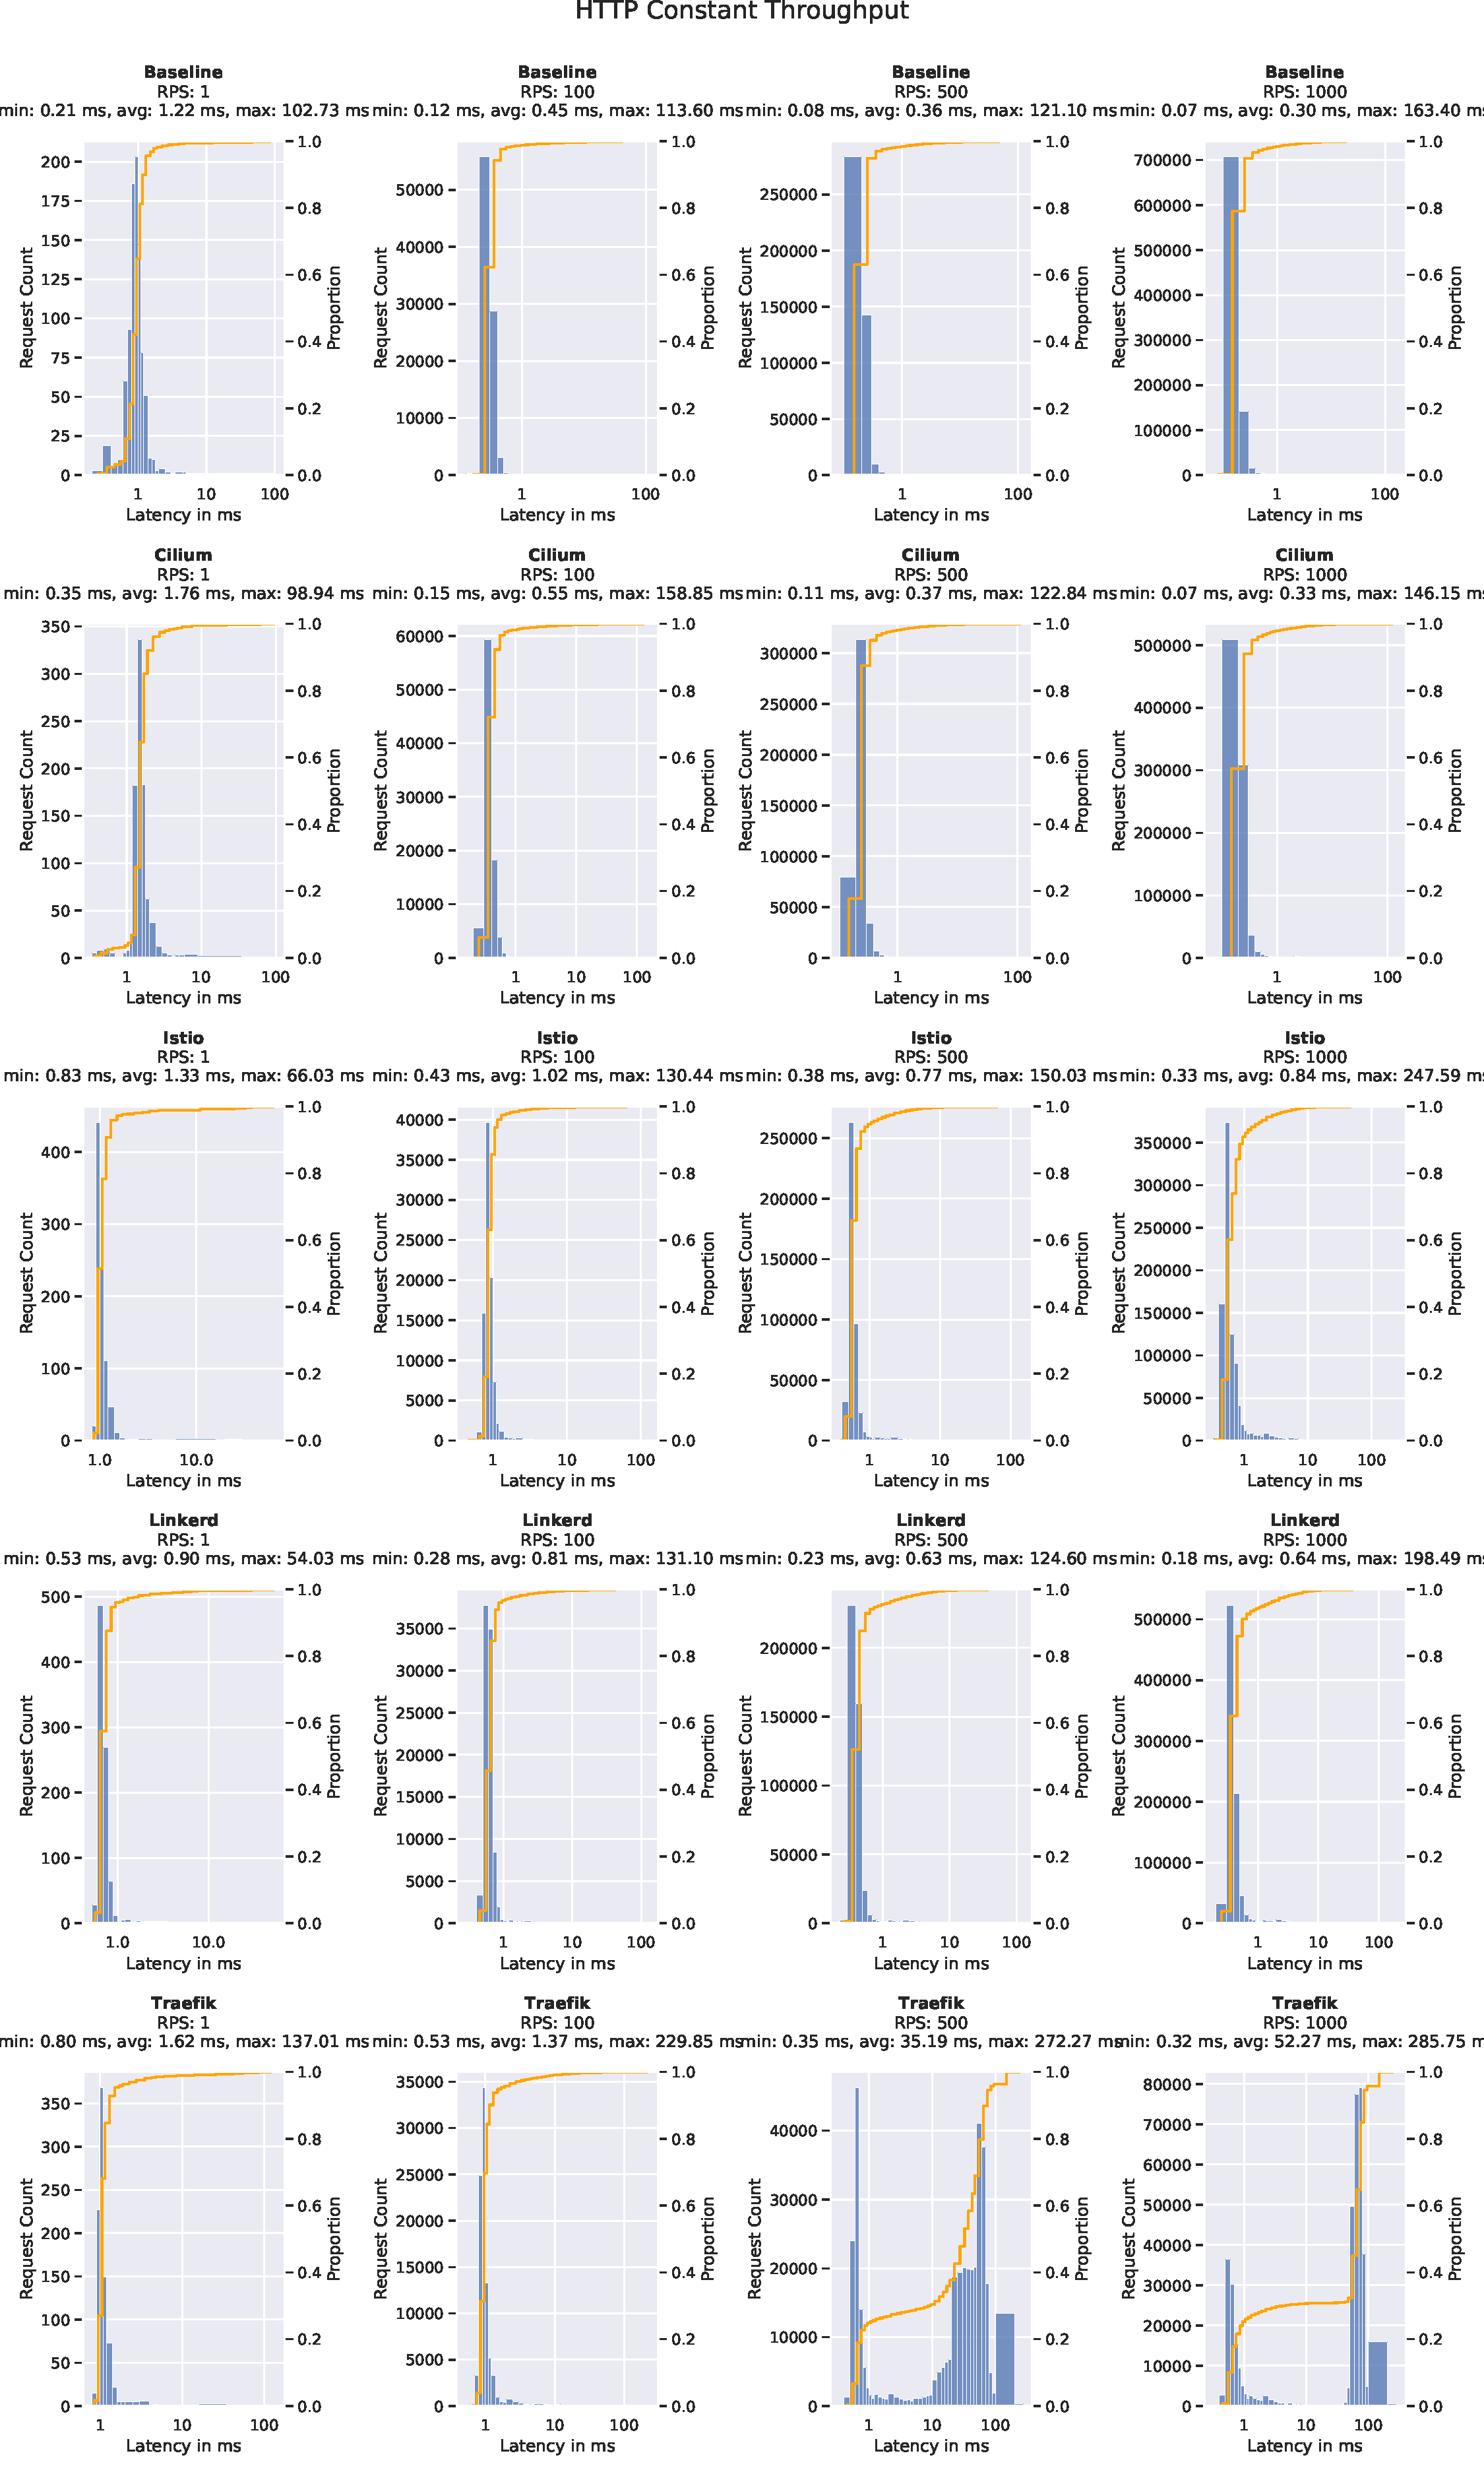
\includegraphics[width=\textwidth,height=\textheight]{5_experimental_evaluation/figures/exp_02-latency-combined-results-offset.pdf}

    \caption{\ref{exp:design:2} - Latency Results}
    
    \label{fig:exp:result:02:latency}
\end{figure}

% How to read all three figures
% - Histogram (latency)
% - Line plot (cpu/mem)
In \cref{fig:exp:result:02:latency} we present a multitude of histograms that display the request latencies measured in each experiment. Every meshed configuration is presented on a row, where each plot on that row contains the histogram for a certain level of throughput. Again, above each histogram we present descriptive statistics and also plot the cumulative density function. In \cref{fig:exp:result:02:cpu} and \cref{fig:exp:result:02:memory} we present the resource utilization metrics obtained from this experiment. Each plot in the illustrations represents a meshed configuration. The y-axis represents the system resource metric such as CPU or memory utilization. The x-axis represents the time delta since the start of the experiment. Note that the line is continuous, since all four different levels of constant throughput are measured one after another. Additionally, each line is coloured and represents a single container on the data path, i.e. target service and proxy (if applicable).

% Results:
% Distribution of traefik changed when peak is hit (~560RPS as in exp1) to bimodal
% Istio/Linkerd max suffering
% - Underlying data/bins (or log plots) show 99p 99.9p suffering
From the histograms \cref{fig:exp:result:02:latency} we can see that for most configurations the distribution stayed very similar. The most significant difference occurs at \textit{Traefik}, where the bimodal distribution occurs at a constant throughput of 500 requests per second and above. This falls in line with the observed behaviour as experienced in \ref{exp:design:1} and indicates a bottleneck of some sort. We can also observe from the descriptive statistics that the maximum values observed in these controlled environments seem to suffer for \textit{Istio}, \textit{Linkerd} and \textit{Traefik} which can be confirmed by taking a closer look at the underlying data that shows higher latency outliers in the tail ends of the spectrum in the 99th and 99.9th percentile.


\begin{figure}[h]
    \centering
    
    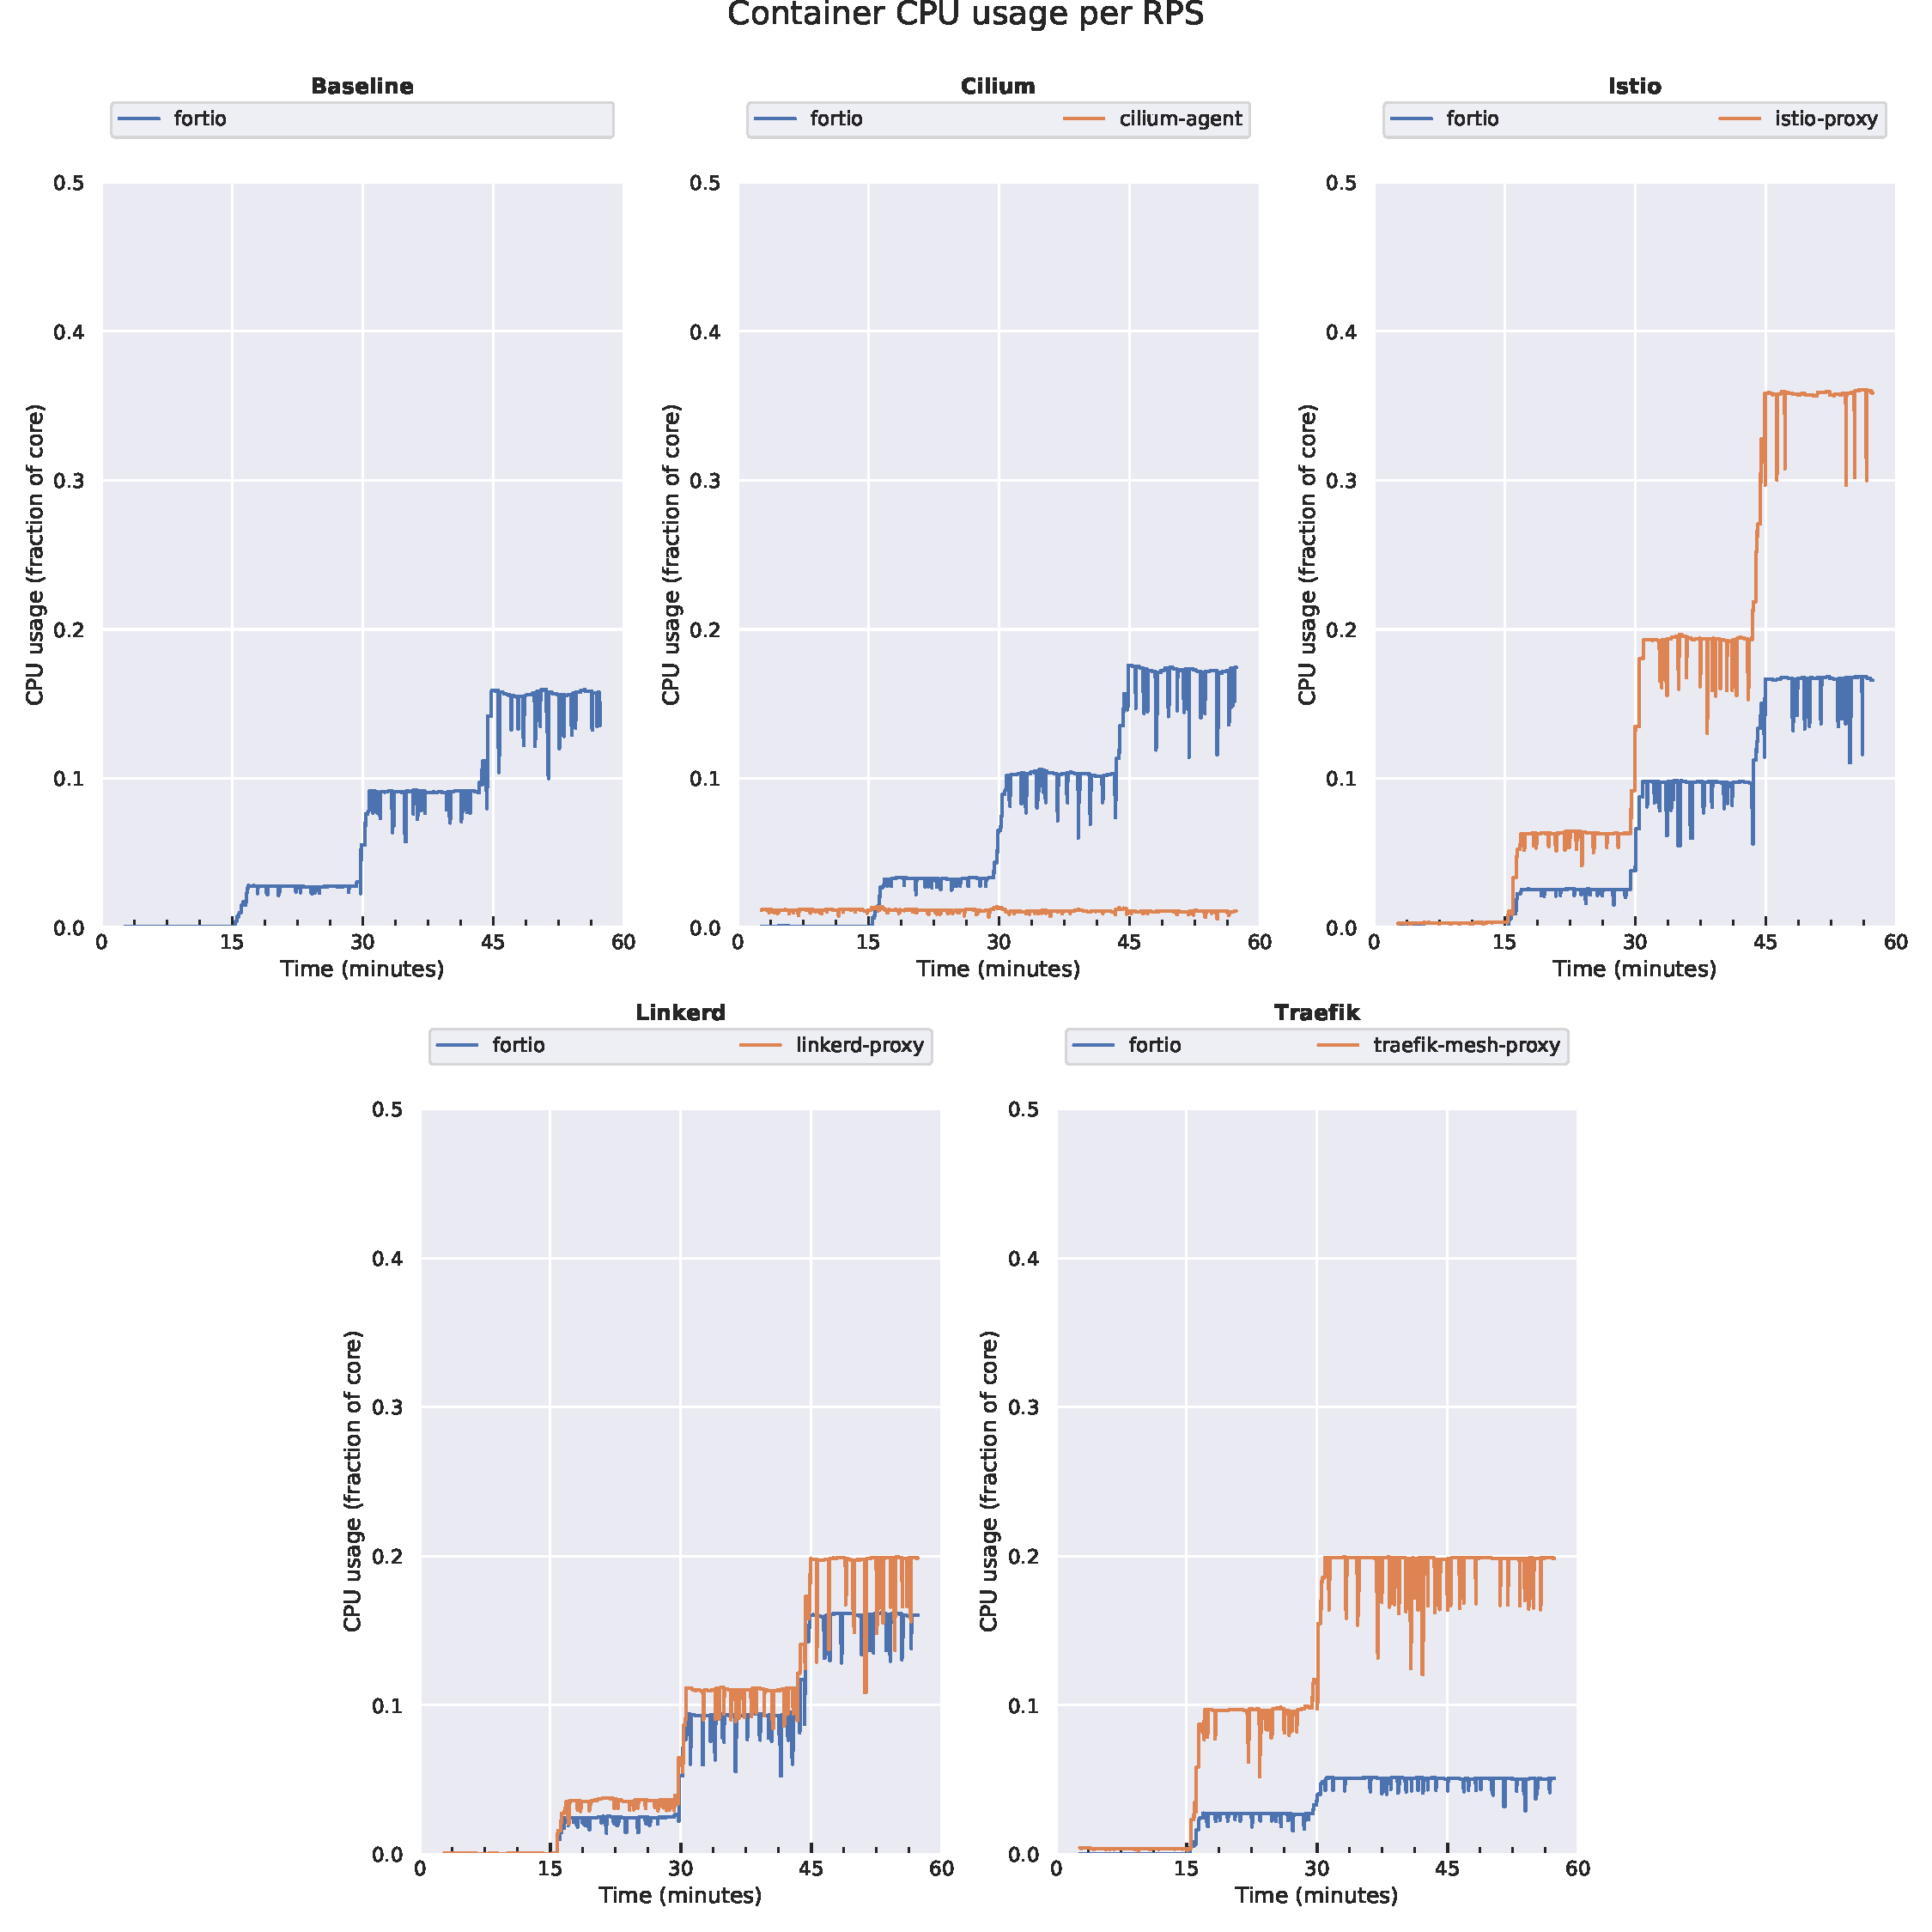
\includegraphics[width=\linewidth]{5_experimental_evaluation/figures/exp_02-cpu-results.pdf}

    \caption{\ref{exp:design:2} - CPU utilization results.}
    
    \label{fig:exp:result:02:cpu}
\end{figure}


% Linar scaling of CPU utilization service
% Istio worst scaling
% Traefik bottleneck at 500
% Memory consumtion similar at all levels
% Linkerd least amount of memory
From the CPU utilization results as depicted in \cref{fig:exp:result:02:cpu} we can observe that the increase in CPU consumption for the target service is linear to the amount of throughput applied. In the results we can observe that \textit{Cilium} seems to consume the least amount of CPU utilization and that it stays stable for each of the workloads. \textit{Istio}, on the other hand, seems to have the worst scaling regarding its CPU utilization. \textit{Linkerd} and \textit{Traefik} seem to scale similarly, however, scaling for the latter stops at the 500 RPS threshold due to its bottleneck. From the memory utilization results as depicted in \cref{fig:exp:result:02:memory} we can observe that \textit{Linkerd} consumes the least amount of memory from all meshed configurations. Another observation is that the memory footprint is similar for each of the workloads, except for the \textit{Traefik} proxy at 1 RPS, which is slightly lower. Again, all observed values are negligible for most environments.


\begin{figure}[h]
    \centering
    
    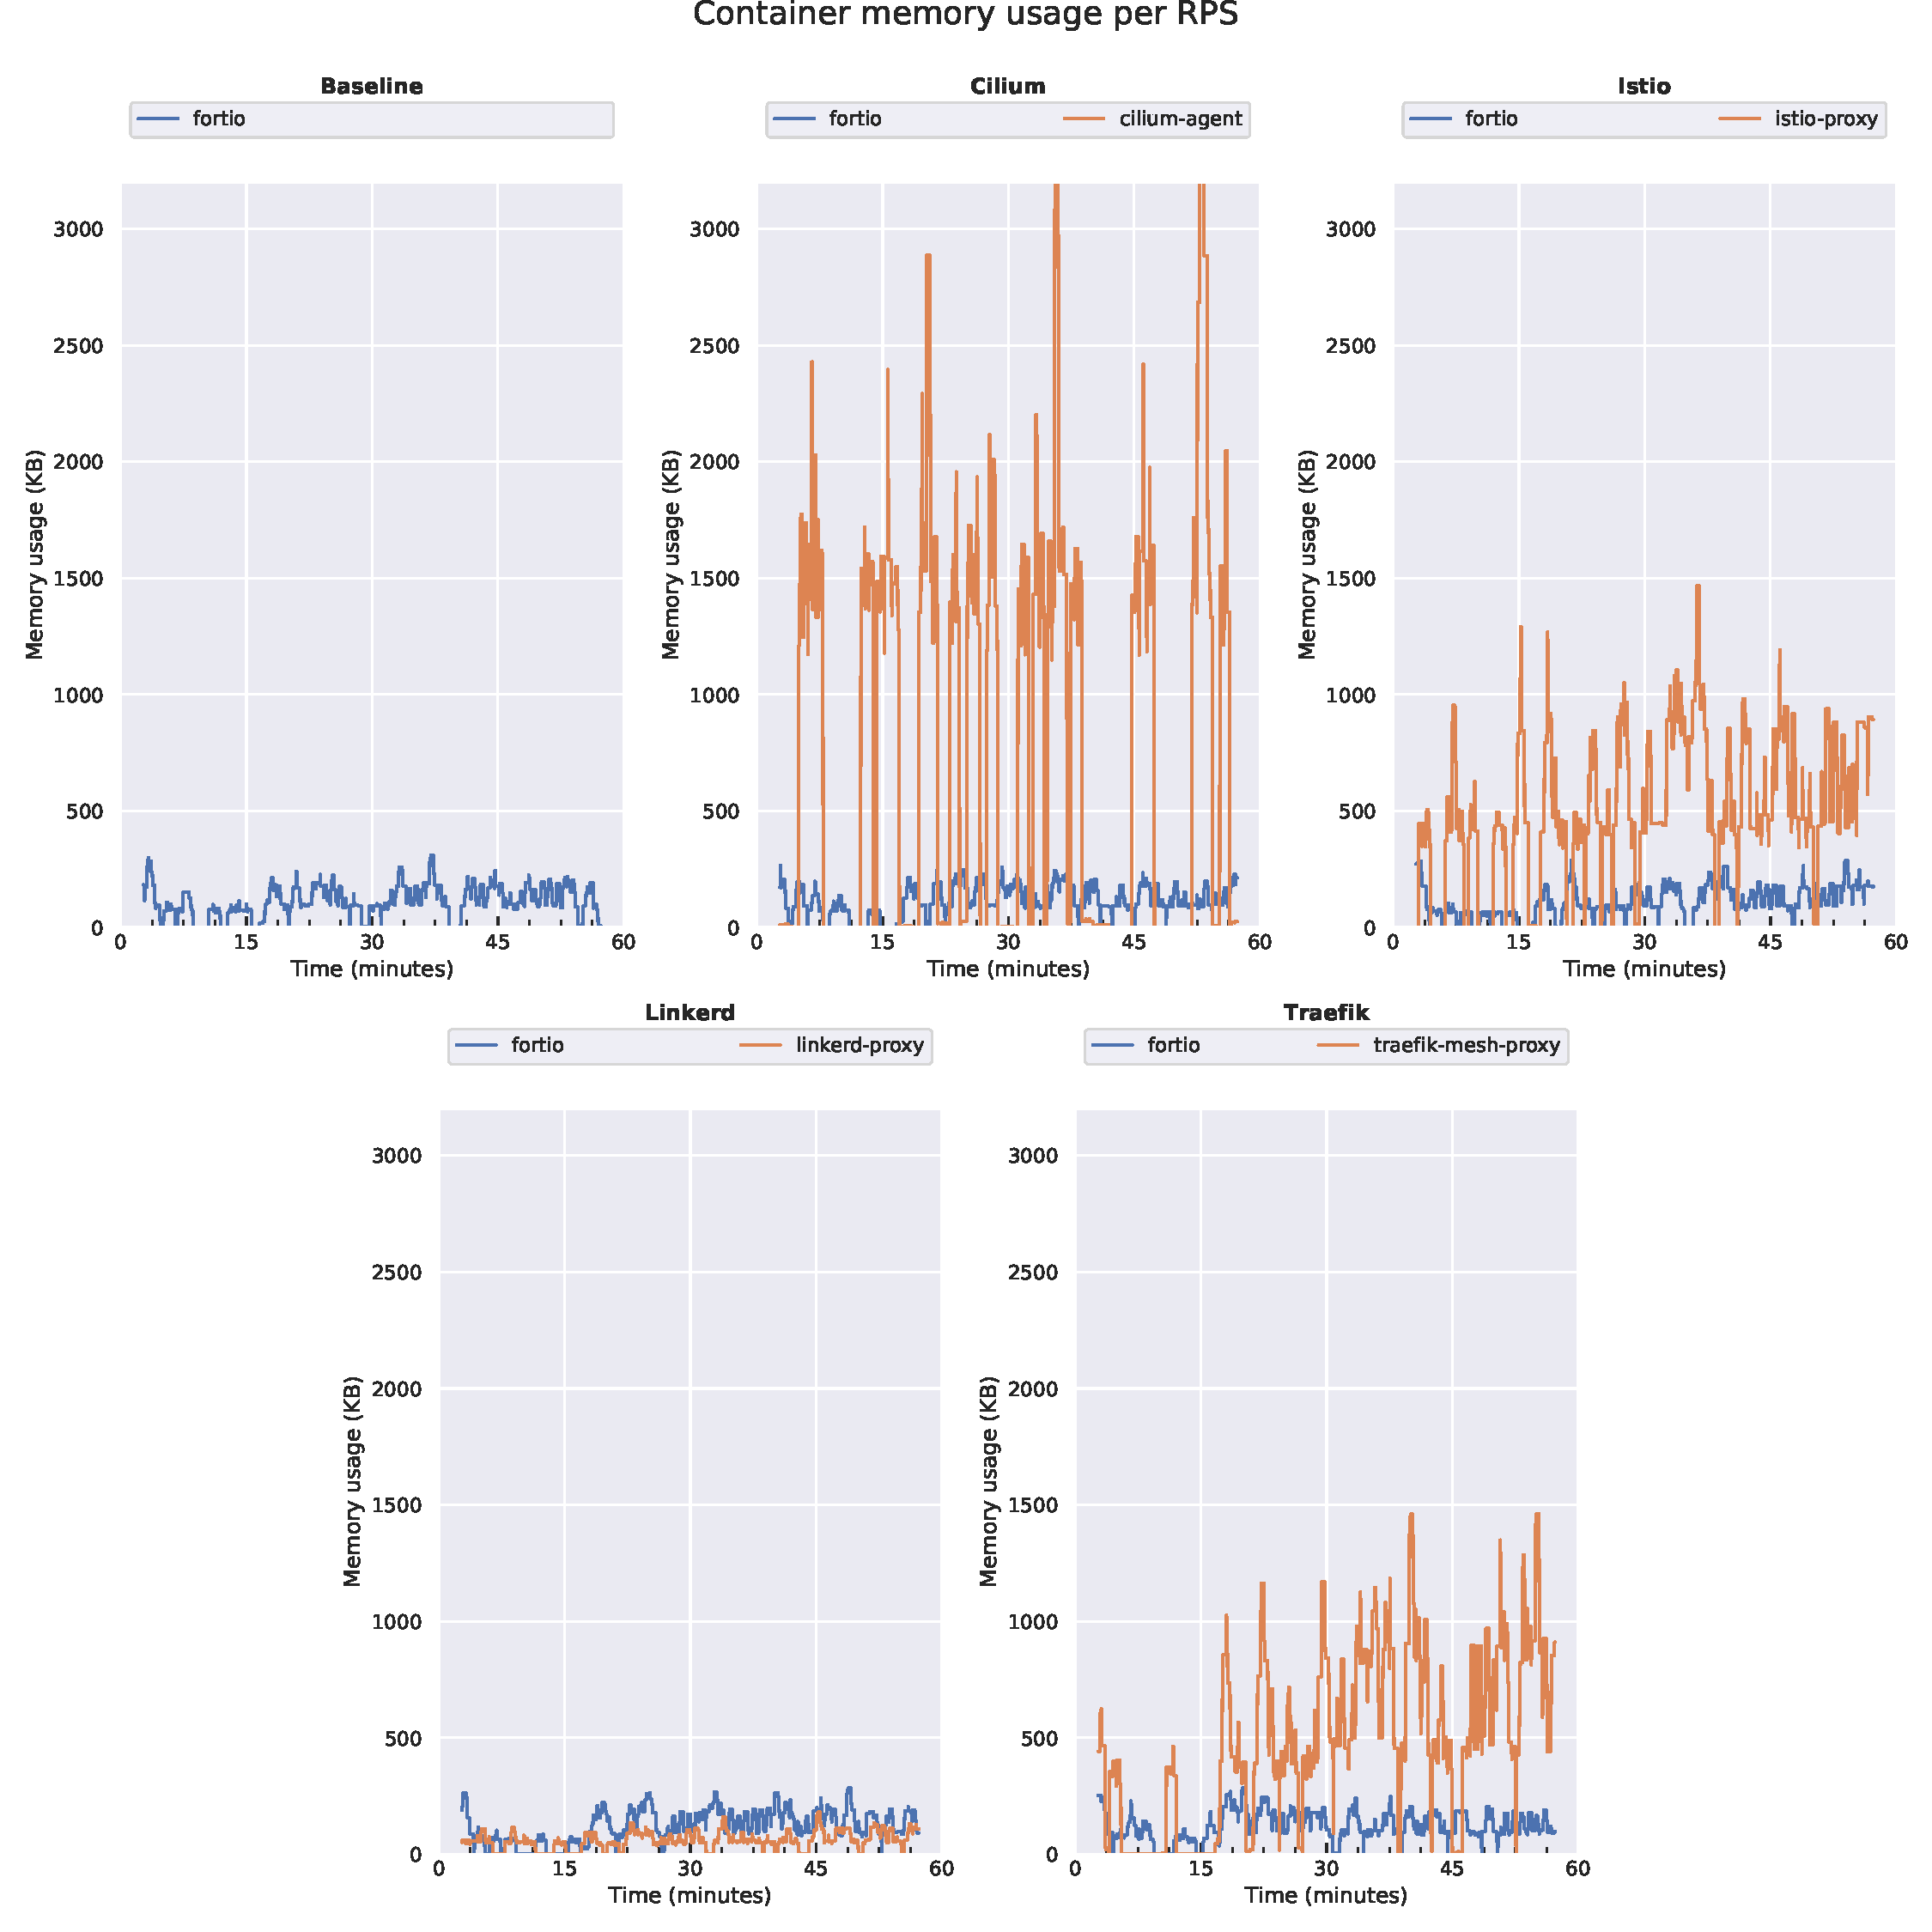
\includegraphics[width=\linewidth]{5_experimental_evaluation/figures/exp_02-mem-results.pdf}

    \caption{\ref{exp:design:2} - memory utilization results.}
    
    \label{fig:exp:result:02:memory}
\end{figure}



\subsubsection{\ref{exp:design:3} - HTTP Payload}
\label{sec:experiments:results:per-experiment:03}

In the third experiment we introduced application payloads. The goal of this experiment is to evaluate the performance of these systems with different payload sizes. The result of this experiment is depicted in \cref{fig:exp:result:03:latency}.

% Explain how to read the figure
\cref{fig:exp:result:03:latency} contains five rows of histogram results. Each of these rows contain the results of a mesh configuration and each of the columns is a result for a given payload size. The first column contains the results of a load test where the target service returns an empty response. The second and third column, however, represent the results of a load test where the target returns a payload of 1 kilobyte and 10 kilobytes respectively as indicated by the plot labels. Additional descriptive statistics are added to each plot without the throughput count as it is static at 100 requests per second for each result in the figure.


\begin{figure}[!t]
    \centering
    
    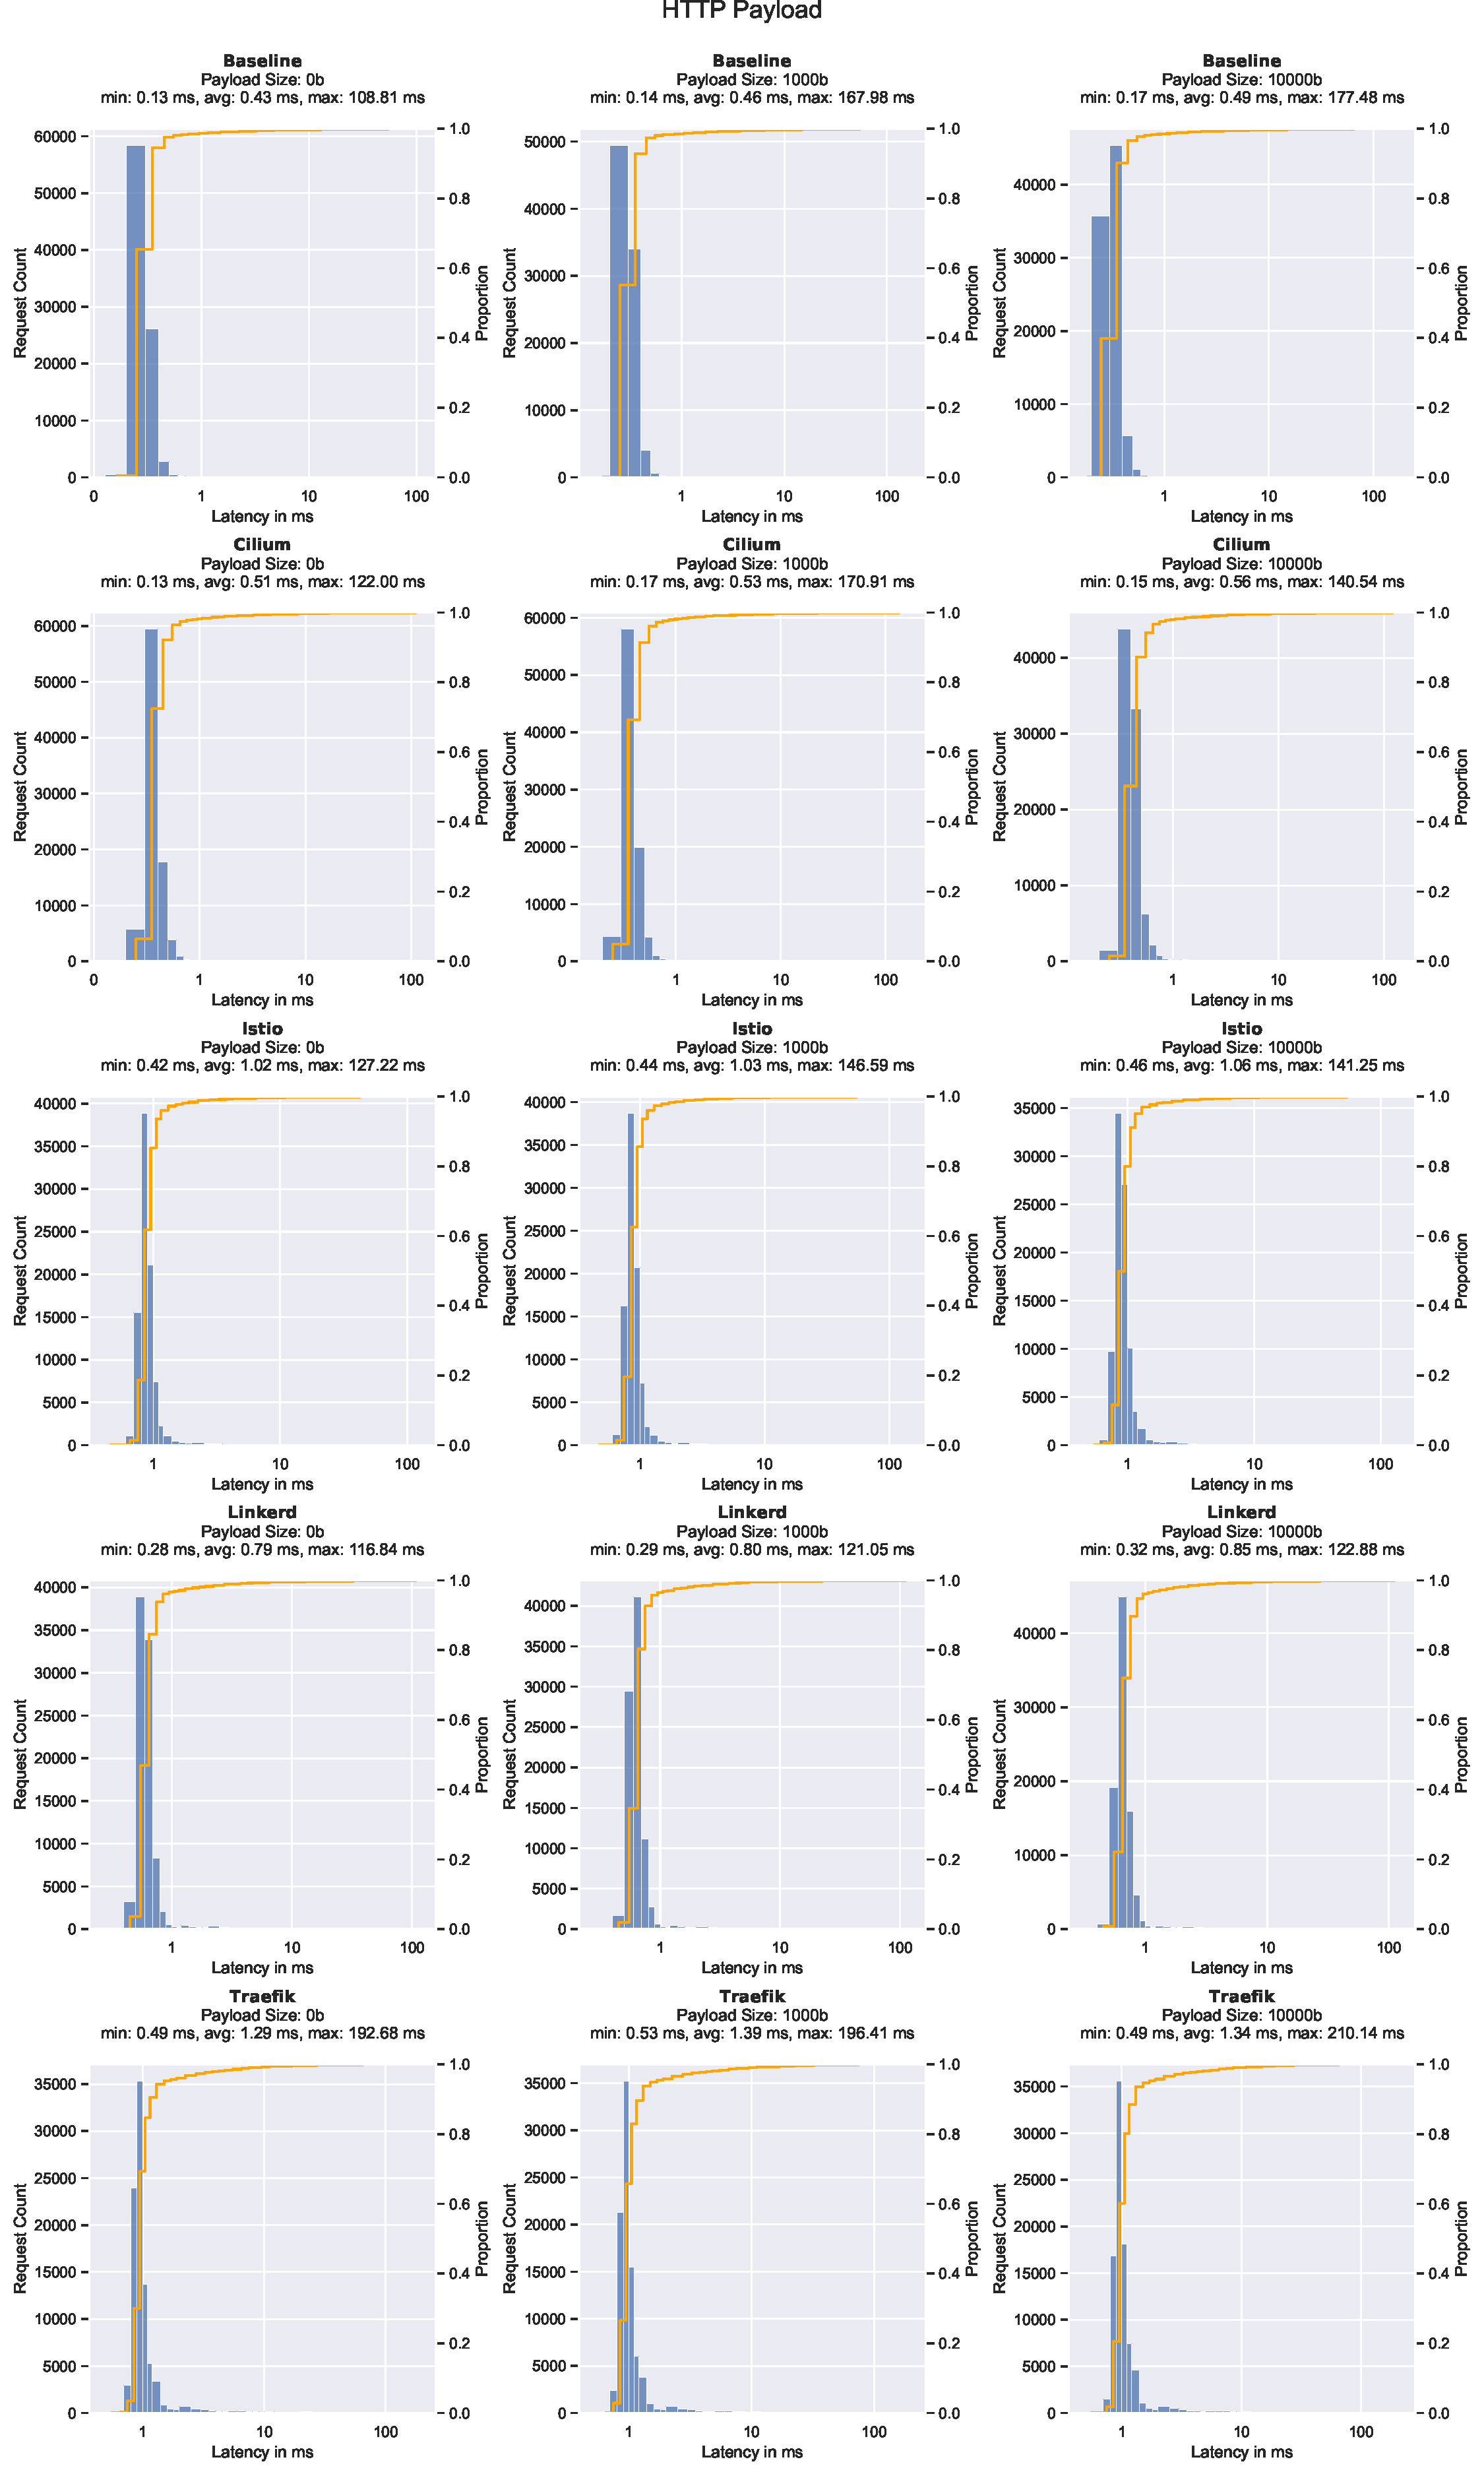
\includegraphics[width=\textwidth,height=\textheight]{5_experimental_evaluation/figures/exp_03-latency-results.pdf}

    \caption{\ref{exp:design:3} - Latency Results}
    
    \label{fig:exp:result:03:latency}
\end{figure}


% Results
% -maximum values higher
% p99.9 p99 similar
From the results of the histograms as depicted in \cref{fig:exp:result:03:latency} we can observe that the distributions remain similar for all the observed payload sizes. In fact, when inspecting the data in finer detail we observe that the tail end is nearly identical and that there is no significant difference in the tail latencies of the 99th and 99.9th percentile. 


\subsubsection{\ref{exp:design:4} - gRPC Maximum Throughput}
\label{sec:experiments:results:per-experiment:04}
% Goal: To evaluate how meshed configurations behave with alternative communication protocols.

The final experiment uses a different type of workload. In this experiment, we aim to evaluate the performance of \gls{sm} systems under alternative application level protocols. The results of this experiment can be seen in \cref{fig:exp:result:04:latency}


\begin{figure}[h]
    \centering
    
    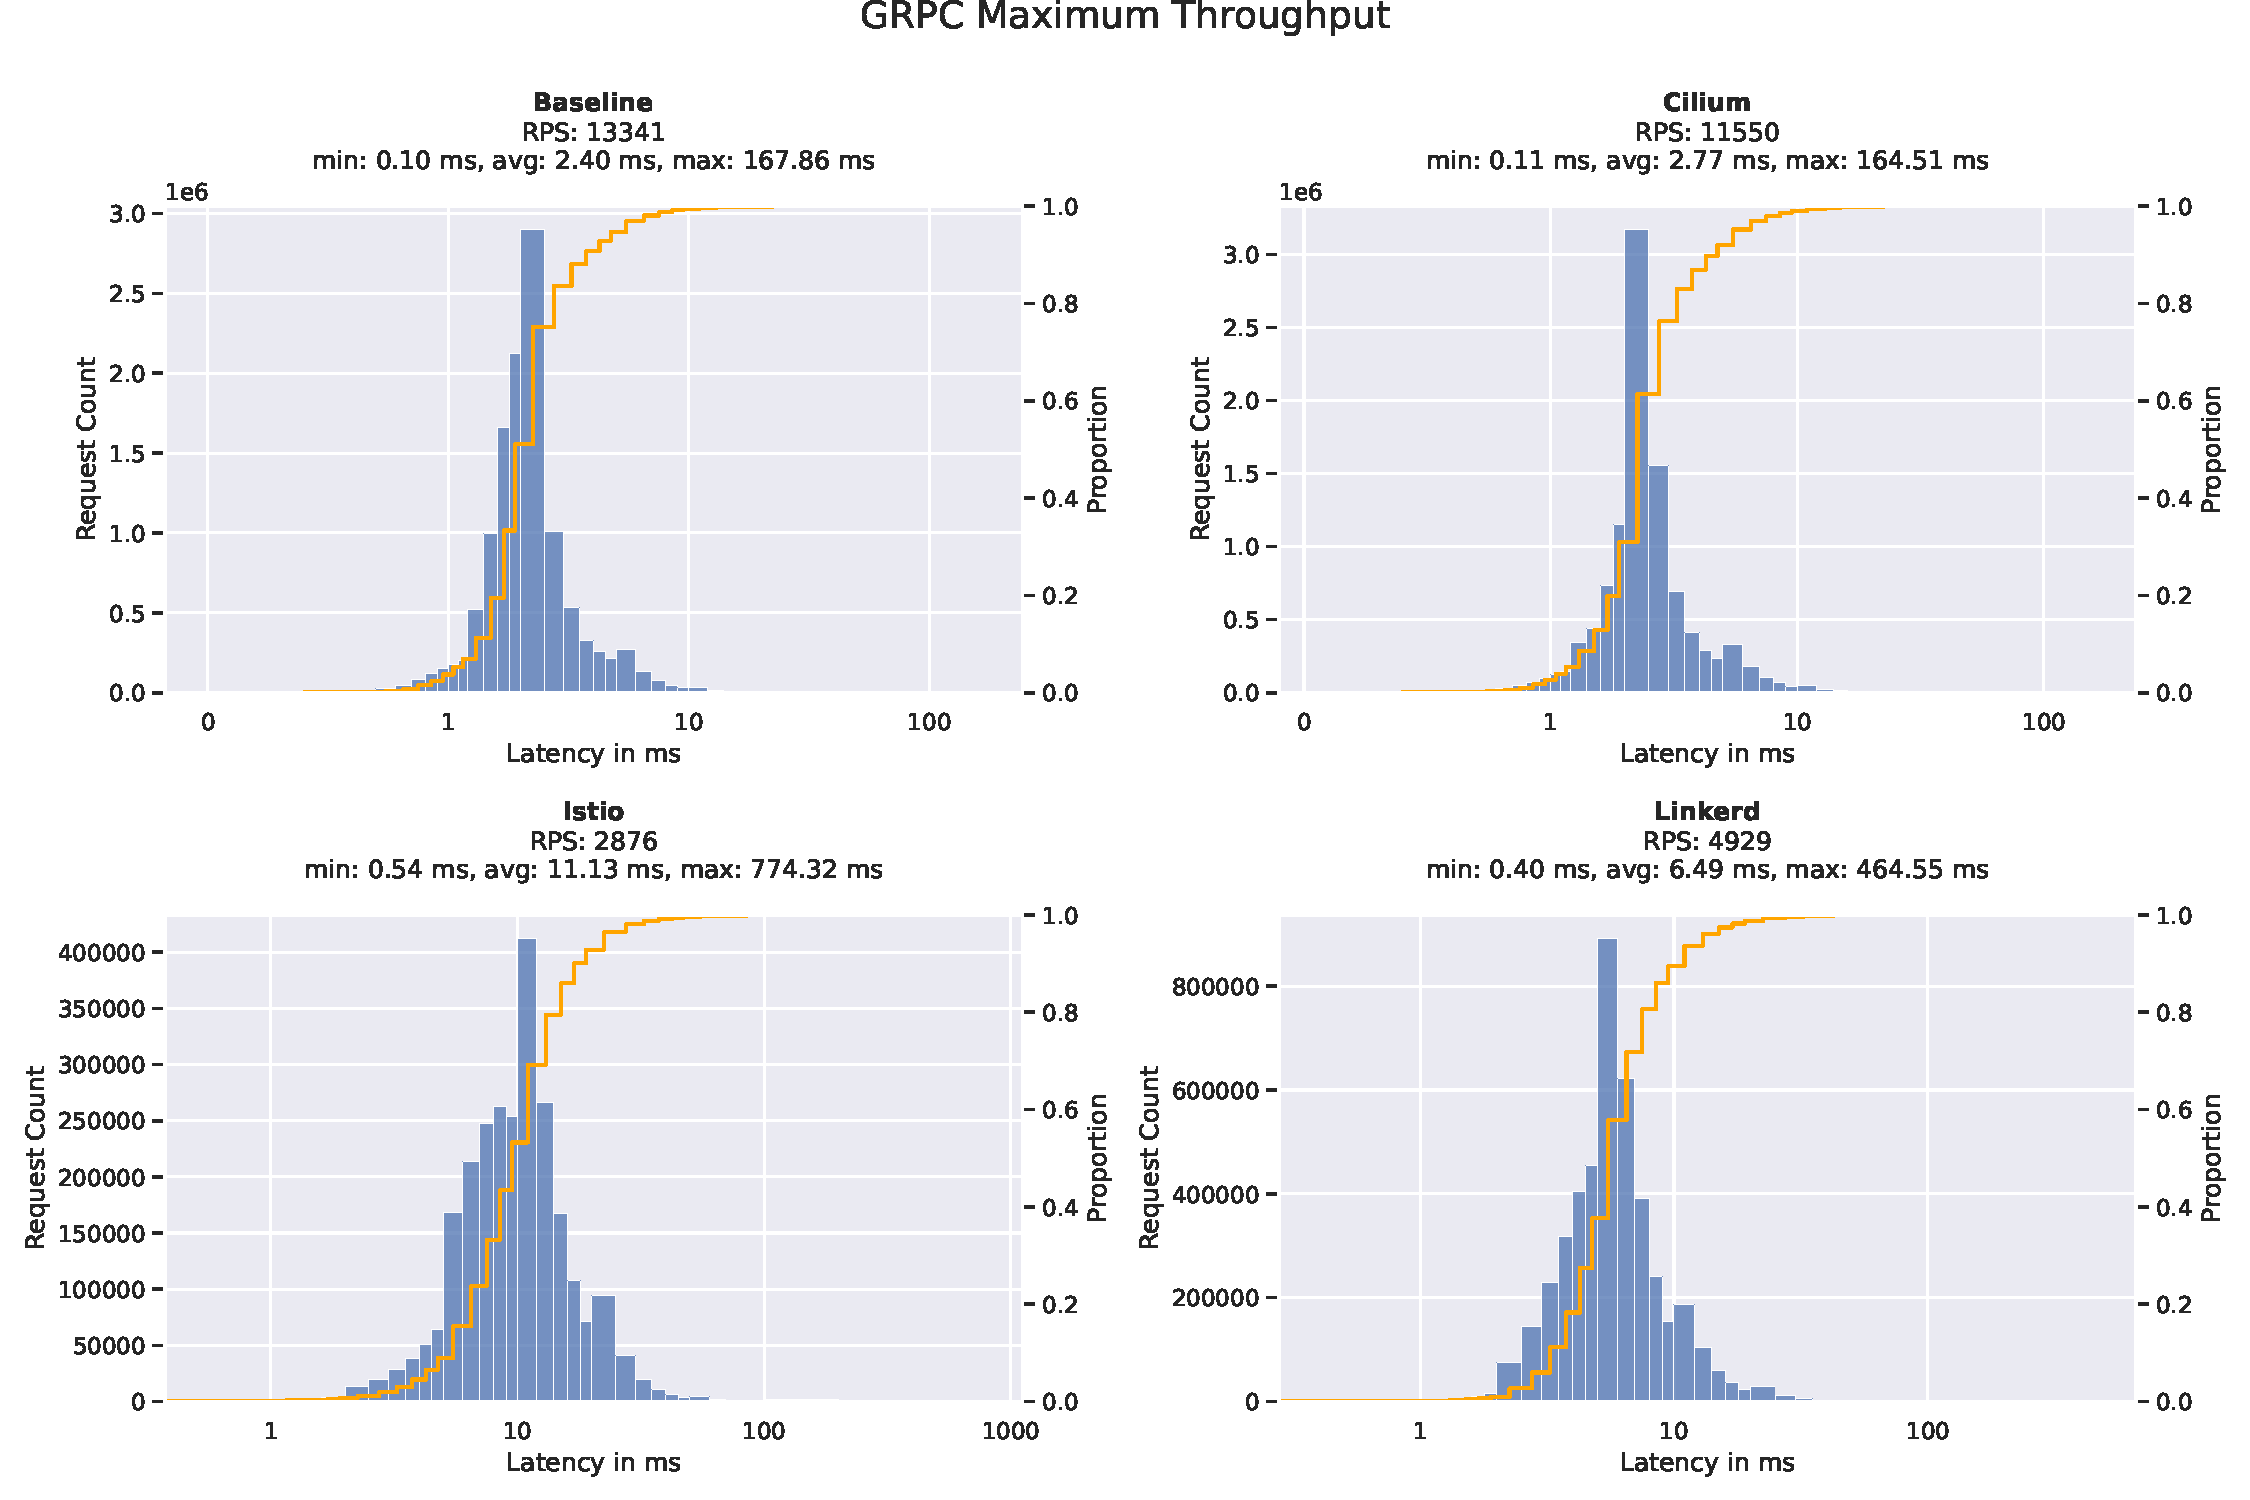
\includegraphics[width=\linewidth]{5_experimental_evaluation/figures/exp_04-latency-results.pdf}

    \caption{\ref{exp:design:4} - latency results.}
    
    \label{fig:exp:result:04:latency}
\end{figure}

% Describe plots
The histograms in \cref{fig:exp:result:04:latency} show the distribution of request latencies of the gRPC workloads for each of the mesh configurations. The y-axis on the left represents the number of requests related to the bars. The y-axis on the right indicates the proportion which is tied to the cumulative distribution function line on top of the histogram. The x-axis is once again a logarithmic axis representing the latency expressed in milliseconds. Additional descriptive metrics are presented above each plot and the actual amount of throughput reached is included as well expressed in requests per second (RPS).

% Results
% - No Traefik -> No support
% - High tail end latencies
% - Drops:
% cilium -13.424%
% istio: -78.442%
% linkerd: -63.053%

% Htpt diff
% cilium QPS diff: -16.827679769486704%
% istio QPS diff: -80.0264142981776%
% linkerd QPS diff: -54.940993873502805%
% traefik QPS diff: -97.38692130213765%
The first observation from this experiment was that the \textit{Traefik} proxy was unable to support and therefore process the gRPC requests, leading to its absence in the depicted results. Furthermore, we can see that for the meshed configurations we again see a decrease in maximum throughput achieved compared to the baseline configuration for all the meshed configurations. Similar to the HTTP experiment as discussed in \cref{sec:experiments:results:per-experiment:01}, we observe that \textit{Cilium} is performing the best out of all meshed configurations regarding its maximum throughput, losing out on $-13.42\%$ compared to the baseline. \textit{Linkerd} and \textit{Istio} have a significant drop compared to the baseline configuration, losing $-54.94\%$ and $-97.39\%$ of the maximum throughput compared to the baseline respectively. An interesting observation can be made is regarding the distributions and tail end latencies of the requests for \textit{Linkerd} and \textit{Istio}. The average requests latencies see a significant increase, with $+170.42\%$ and $+363.75\%$ compared to the baseline average respectively. This trend continues for the tail end latencies and maximum values observed as well indicating that the proxies introduce a notable performance overhead.

% istio ~38 p99
% linkerd ~22 p99
\section{Summary}
\label{sec:experiments:summary}


